\documentclass[]{book}
\usepackage{lmodern}
\usepackage{amssymb,amsmath}
\usepackage{ifxetex,ifluatex}
\usepackage{fixltx2e} % provides \textsubscript
\ifnum 0\ifxetex 1\fi\ifluatex 1\fi=0 % if pdftex
  \usepackage[T1]{fontenc}
  \usepackage[utf8]{inputenc}
\else % if luatex or xelatex
  \ifxetex
    \usepackage{mathspec}
    \usepackage{xltxtra,xunicode}
  \else
    \usepackage{fontspec}
  \fi
  \defaultfontfeatures{Mapping=tex-text,Scale=MatchLowercase}
  \newcommand{\euro}{€}
\fi
% use upquote if available, for straight quotes in verbatim environments
\IfFileExists{upquote.sty}{\usepackage{upquote}}{}
% use microtype if available
\IfFileExists{microtype.sty}{%
\usepackage{microtype}
\UseMicrotypeSet[protrusion]{basicmath} % disable protrusion for tt fonts
}{}
\usepackage{color}
\usepackage{fancyvrb}
\newcommand{\VerbBar}{|}
\newcommand{\VERB}{\Verb[commandchars=\\\{\}]}
\DefineVerbatimEnvironment{Highlighting}{Verbatim}{commandchars=\\\{\}}
% Add ',fontsize=\small' for more characters per line
\newenvironment{Shaded}{}{}
\newcommand{\KeywordTok}[1]{\textbf{{#1}}}
\newcommand{\DataTypeTok}[1]{\textcolor[rgb]{0.50,0.00,0.00}{{#1}}}
\newcommand{\DecValTok}[1]{\textcolor[rgb]{0.00,0.00,1.00}{{#1}}}
\newcommand{\BaseNTok}[1]{\textcolor[rgb]{0.00,0.00,1.00}{{#1}}}
\newcommand{\FloatTok}[1]{\textcolor[rgb]{0.50,0.00,0.50}{{#1}}}
\newcommand{\CharTok}[1]{\textcolor[rgb]{1.00,0.00,1.00}{{#1}}}
\newcommand{\StringTok}[1]{\textcolor[rgb]{0.87,0.00,0.00}{{#1}}}
\newcommand{\CommentTok}[1]{\textcolor[rgb]{0.50,0.50,0.50}{\textit{{#1}}}}
\newcommand{\OtherTok}[1]{{#1}}
\newcommand{\AlertTok}[1]{\textcolor[rgb]{0.00,1.00,0.00}{\textbf{{#1}}}}
\newcommand{\FunctionTok}[1]{\textcolor[rgb]{0.00,0.00,0.50}{{#1}}}
\newcommand{\RegionMarkerTok}[1]{{#1}}
\newcommand{\ErrorTok}[1]{\textcolor[rgb]{1.00,0.00,0.00}{\textbf{{#1}}}}
\newcommand{\NormalTok}[1]{{#1}}
\usepackage{graphicx}
\makeatletter
\def\maxwidth{\ifdim\Gin@nat@width>\linewidth\linewidth\else\Gin@nat@width\fi}
\def\maxheight{\ifdim\Gin@nat@height>\textheight\textheight\else\Gin@nat@height\fi}
\makeatother
% Scale images if necessary, so that they will not overflow the page
% margins by default, and it is still possible to overwrite the defaults
% using explicit options in \includegraphics[width, height, ...]{}
\setkeys{Gin}{width=\maxwidth,height=\maxheight,keepaspectratio}
\ifxetex
  \usepackage[setpagesize=false, % page size defined by xetex
              unicode=false, % unicode breaks when used with xetex
              xetex]{hyperref}
\else
  \usepackage[unicode=true]{hyperref}
\fi
\hypersetup{breaklinks=true,
            bookmarks=true,
            pdfauthor={},
            pdftitle={HoH: CSL373/CSL633 Labs},
            colorlinks=true,
            citecolor=blue,
            urlcolor=blue,
            linkcolor=magenta,
            pdfborder={0 0 0}}
\urlstyle{same}  % don't use monospace font for urls
\setlength{\parindent}{0pt}
\setlength{\parskip}{6pt plus 2pt minus 1pt}
\setlength{\emergencystretch}{3em}  % prevent overfull lines
\setcounter{secnumdepth}{5}

\title{HoH: CSL373/CSL633 Labs\\\vspace{0.5em}{\large \emph{What's the best way for learning OS? Create one!}}}
\date{Jan 1, 2015}

\begin{document}
\maketitle

Also available in \href{index.pdf}{pdf},
\href{index.slides.html}{slides}. \href{index.beamer.pdf}{beamer}.
\href{index.tex}{latex}.

\section*{Introduction}\label{introduction}
\addcontentsline{toc}{section}{Introduction}

\subsubsection*{Introduction}\label{introduction-1}
\addcontentsline{toc}{subsubsection}{Introduction}

Hello! I'm Alice. I am your TA for this course.

In this series, you will join forces with me, and together, we will
build a \emph{kernel from the scratch}. We both will be working on this
kernel.

I'll do some coding in a branch, and ask you to implement some
functionality. You can get my code by merging the branch with yours, and
implement the functionality I asked. Once you implement it and commit
the changes in your repository, I'll again work on the kernel on some
other branch..

\subsubsection*{Status so far - our kernel boots into C
code}\label{status-so-far---our-kernel-boots-into-c-code}
\addcontentsline{toc}{subsubsection}{Status so far - our kernel boots
into C code}

So far, I have managed to write:
\href{http://wiki.osdev.org/Bare_bones}{See osdev barebones}

\begin{enumerate}
\def\labelenumi{\arabic{enumi}.}
\item
  x86/boot.S : containing seven lines of 32-bit x86 assembly
  instructions to:

  \begin{itemize}
  \item
    set the stack pointer,

\begin{verbatim}
   movl  $tmpstack_bottom, %esp
\end{verbatim}
  \item
    clear flags,

\begin{verbatim}
   pushl $0
   popf
\end{verbatim}
  \item
    call the C function

\begin{verbatim}
   call  core_boot
\end{verbatim}
  \item
    enter infinite loop

\begin{verbatim}
   cli
 loop:
   hlt
   jmp   loop
\end{verbatim}
  \end{itemize}
\item
  x86/main.cc : a C function which does nothing

\begin{Shaded}
\begin{Highlighting}[]
 \KeywordTok{extern} \StringTok{"C"} \DataTypeTok{void} \NormalTok{core_boot()\{}
 \NormalTok{\}}
\end{Highlighting}
\end{Shaded}
\end{enumerate}

\subsubsection*{make}\label{make}
\addcontentsline{toc}{subsubsection}{make}

\begin{itemize}
\item
  Syntax:

\begin{Shaded}
\begin{Highlighting}[]
\KeywordTok{bash}\NormalTok{$ make }\KeywordTok{<}\NormalTok{target}\KeywordTok{>} \NormalTok{B=}\KeywordTok{<}\NormalTok{release/debug}\KeywordTok{>}
\KeywordTok{where} \NormalTok{target =}
  \KeywordTok{iso}      \NormalTok{: create boot cd}
  \KeywordTok{exe}      \NormalTok{: build kernel (default)}
  \KeywordTok{qemu}     \NormalTok{: run qemu}
  \KeywordTok{qemu-gdb} \NormalTok{: qemu with gdb}
\end{Highlighting}
\end{Shaded}
\item
  Usage: make iso / make qemu / make qemu-gdb B=debug
\item
  Try `make qemu-direct' and `make qemu-gdb-direct B=debug' if you face
  any issues.
\end{itemize}

\subsubsection*{On Boot}\label{on-boot}
\addcontentsline{toc}{subsubsection}{On Boot}

\begin{itemize}
\itemsep1pt\parskip0pt\parsep0pt
\item
  CPU sets cs:ip to 0xffff:0x0000 and starts executing code from this
  location(BIOS ROM is memory mapped at this location. When CPU tries to
  load the instruction from this location, cache and memory will be
  bypassed, and instructions will be directly loaded from ROM).
\item
  \emph{CPU starts executing BIOS code directly from ROM.}
\item
  BIOS code initializes cache, RAM and other peripherals
\item
  BIOS code installs its handlers by modifying Interrupt descriptor
  table(IDT) to provide services for bootloader
\item
  BIOS loads the boot loader(grub2) code from the boot disk at
  0x0000:0x7c00 and jump to it. Now, \emph{CPU starts executing boot
  loader code(grub2)}.
\item
  (specific to grub2): grub2 uses bios provided interrupt handlers to
  load it's configuration file /boot/grub/grub2.cfg and gets the path of
  kernel to be loaded, and the kernel is multiboot standard compatible -
  and grub2 switches the CPU to 32 bit mode.
\item
  Bootloader(grub2) loads initial part of kernel containing ELF header
  from the disk (using BIOS provided interrupt handlers) into RAM
\item
  grub2 scans kernel's initial part for `multiboot header' to know the
  interface expected from the kernel - for ex: multiboot version.
\item
  Bootloader reads the ELF header and loads each section of kernel from
  disk into corresponding address in RAM(as mentioned in ELF header)
\item
  Bootloader jumps to the starting address mentioned in kernel's ELF
  header(usually \_start)
\item
  \emph{CPU starts executing kernel code}(\_start).
\end{itemize}

\subsubsection*{Analyzing tracefile}\label{analyzing-tracefile}
\addcontentsline{toc}{subsubsection}{Analyzing tracefile}

I've enabled qemu's instruction tracing. So after executing `make qemu',
a trace file created named qemu.log in the current working directory.

When looking at the tracefile(qemu.log), please skip the initial bios
instructions

\begin{verbatim}
     ----------------
     IN:
     0xfffffff0:  ljmp   $0xf000,$0xe05b
\end{verbatim}

and also skip the bootloader code,

\begin{verbatim}
     ----------------
     IN:
     0x00007c00:  call   0x7c03
\end{verbatim}

\subsubsection*{Our kernel's instruction
trace}\label{our-kernels-instruction-trace}
\addcontentsline{toc}{subsubsection}{Our kernel's instruction trace}

Towards the end you can see our kernel's instruction trace. For example:

\begin{verbatim}
     ----------------
     IN:
     0x00100050:  mov    $0x104080,%esp
     0x00100055:  push   $0x0
     0x00100057:  popf
     0x00100058:  call   0x1040a0
     ----------------
     IN: core_boot
     0x001040a0:  repz ret
     0x0010005d:  cli
     0x0010005e:  hlt
\end{verbatim}

\subsubsection*{Boot our kernel from your
laptop}\label{boot-our-kernel-from-your-laptop}
\addcontentsline{toc}{subsubsection}{Boot our kernel from your laptop}

Optional:
\href{http://www.gnu.org/software/grub/manual/multiboot/multiboot.pdf}{Multiboot
specification} specifies the interface between boot loader(eg: grub) and
the kernel. You can also boot our kernel from your laptop, by using any
multiboot combatible boot loader.

For example: On grub2, I press `c' to enter command prompt, and type:

\begin{verbatim}
     (grub2) multiboot (hd0,msdos5)/home/alice/hohlabs/_tmp/hoh.exe
     (grub2) boot
\end{verbatim}

\section*{Setup}\label{setup}
\addcontentsline{toc}{section}{Setup}

So here's what you should do:

\subsubsection*{Tools}\label{tools}
\addcontentsline{toc}{subsubsection}{Tools}

Please ensure you have latest version of:

\begin{itemize}
\itemsep1pt\parskip0pt\parsep0pt
\item
  qemu (package: qemu qemu-system)
\item
  g++ (package: g++-multilib \textgreater{}=4.7)
\item
  git (package: git-all)
\item
  grub2 (package: grub2 grub-pc-bin)
\item
  boost library (package: libboost-all-dev)
\item
  xorriso (to create iso image. Otherwise you'll get a warning that )
\item
  coreutils(for makefile)
\end{itemize}

In debian/ubuntu, do:

\begin{Shaded}
\begin{Highlighting}[]
   \KeywordTok{bash}\NormalTok{$ sudo apt-get install qemu qemu-system g++-multilib git-all grub2 grub-pc-bin libboost-all-dev xorriso}
\end{Highlighting}
\end{Shaded}

You can see
\href{http://www.cse.iitd.ac.in/~sbansal/os/tools.html}{tools} to know
more about these tools.

\subsubsection*{Clone the repository}\label{clone-the-repository}
\addcontentsline{toc}{subsubsection}{Clone the repository}

Since we both will work on this kernel, we need to have a version
control system. We'll use git as our version control system. Please
clone the repository to your local directory

\begin{Shaded}
\begin{Highlighting}[]
     \KeywordTok{user@host}\NormalTok{:~$ git clone ssh://}\KeywordTok{<}\NormalTok{user}\KeywordTok{>}\NormalTok{@palasi.cse.iitd.ac.in/misc/research/teaching/sbansal/csl373/hohlabs.git}
     \KeywordTok{user@host}\NormalTok{:~$ cd hohlabs}
     \KeywordTok{user@host}\NormalTok{:~/hohlabs$}
\end{Highlighting}
\end{Shaded}

\subsubsection*{Procedure}\label{procedure}
\addcontentsline{toc}{subsubsection}{Procedure}

For each parts, do

\begin{enumerate}
\def\labelenumi{\arabic{enumi}.}
\item
  Please get the changes done by Alice by merging the corresponding
  branch to your master branch

\begin{Shaded}
\begin{Highlighting}[]
 \KeywordTok{user@host}\NormalTok{:~/hohlabs$ git pull}
 \KeywordTok{user@host}\NormalTok{:~/hohlabs$ git merge origin/}\KeywordTok{<}\NormalTok{branch_name}\KeywordTok{>}
\end{Highlighting}
\end{Shaded}

  For example, to get first part, do:

\begin{Shaded}
\begin{Highlighting}[]
 \KeywordTok{user@host}\NormalTok{:~/hohlabs$ git pull}
 \KeywordTok{user@host}\NormalTok{:~/hohlabs$ git merge origin/vgatext}
\end{Highlighting}
\end{Shaded}
\item
  \emph{Modify the files under the directory ``labs'' only } to add the
  missing functionality. For example, for the first part, you should
  modify the function writechar in labs/vgatext.h

\begin{Shaded}
\begin{Highlighting}[]
 \KeywordTok{user@host}\NormalTok{:~/hohlabs$ git pull}
 \KeywordTok{user@host}\NormalTok{:~/hohlabs$ vim labs/vgatext.h}
\end{Highlighting}
\end{Shaded}

  Test your code by:

\begin{Shaded}
\begin{Highlighting}[]
 \KeywordTok{user@host}\NormalTok{:~/hohlabs$ make qemu}
\end{Highlighting}
\end{Shaded}

  (Optional) To debug:

  \begin{itemize}
  \item
    From first terminal:

\begin{Shaded}
\begin{Highlighting}[]
\KeywordTok{user@host}\NormalTok{:~/hohlabs$ make qemu B=debug}
\end{Highlighting}
\end{Shaded}
  \item
    From another terminal:

\begin{Shaded}
\begin{Highlighting}[]
   \KeywordTok{user@host}\NormalTok{:~/hohlabs$ gdb}
\end{Highlighting}
\end{Shaded}
  \end{itemize}

  In gdb, you can set break point for example '\_start'

\begin{verbatim}
   (gdb) break _start
   (gdb) ni
   (gdb) continue
\end{verbatim}
\item
  Commit your changes in your local repository

\begin{Shaded}
\begin{Highlighting}[]
   \KeywordTok{user@host}\NormalTok{:~/hohlabs$ git add -p labs/}
   \KeywordTok{user@host}\NormalTok{:~/hohlabs$ git commit -m }\StringTok{"your log message"}

   \CommentTok{#Advanced: git add labs/ ; git commit -m "commit message" ; git stash ; ....  now do pull/merge .... ; git stash pop;}
\end{Highlighting}
\end{Shaded}
\item
  Do submit your code so far. (resubmissions are allowed)
\end{enumerate}

\subsubsection*{Submission}\label{submission}
\addcontentsline{toc}{subsubsection}{Submission}

\begin{itemize}
\itemsep1pt\parskip0pt\parsep0pt
\item
  To submit the assignment, from palasi:

  \begin{itemize}
  \item
    make sure your changes are available in palasi. Skip this step, if
    you're working in GCL.
  \item
    submit your changes in palasi using:

\begin{Shaded}
\begin{Highlighting}[]
   \KeywordTok{user@palasi}\NormalTok{:~/hohlabs$ os-submit-lab }\KeywordTok{<}\NormalTok{labid}\KeywordTok{>}
\end{Highlighting}
\end{Shaded}
  \end{itemize}
\item
  Can be submitted from palasi only.
\item
  Resubmissions are allowed.
\item
  For late penalty calculations, we only consider your submission using
  os-submit-lab ( It is possible to change git commit history and
  filesystem modification time)
\item
  Make sure you check your submission is correct by using:
  os-get-submission
\end{itemize}

\begin{center}\rule{0.5\linewidth}{\linethickness}\end{center}

\chapter{Primitives}\label{primitives}

\subsubsection*{Overview}\label{overview}
\addcontentsline{toc}{subsubsection}{Overview}

In this first part, we'll look into basic primitives required for
writing an OS.

\begin{itemize}
\itemsep1pt\parskip0pt\parsep0pt
\item
  Evaluation:

  \begin{itemize}
  \item
    Code component:

    \begin{itemize}
    \itemsep1pt\parskip0pt\parsep0pt
    \item
      \emph{NOTHING : 0 } Not working
    \item
      \emph{PARTIAL : 1 } Partial/buggy - TA is able to find atleast one
      bug in your code
    \item
      \emph{TYPO : 1.5} Code is not clean
    \item
      \emph{CORRECT : 2 } Working code
    \end{itemize}
  \item
    Viva component:

    \begin{itemize}
    \itemsep1pt\parskip0pt\parsep0pt
    \item
      \emph{FLAGGED : 0 } Can not explain his/her own code
    \item
      \emph{JUST\_IMPLEMENTED : 1 } can explain his/her own code but
      can't explain Alice's code
    \item
      \emph{KNOWS\_WHY : 2 } can explain his/her own code + Alice's code
    \end{itemize}
  \item
    Marks for each part is computed by following equation:
    \[ Marks = (W_d * D + W_v * V) \]
  \item
    For 1.1-1.3: \(W_d = 0.25\) and \(W_v = 0.25\)
  \item
    For 1.4-1.7: \(W_d = 0.40\) and \(W_v = 0.10\)
  \item
    For 1.8: \(W_d = 1.20\) and \(W_v = 0.30\)
  \item
    For 1.9: \(W_d = 0.80\) and \(W_v = 0.20\)
  \item
    For 1.10: \(W_d = 1.20\) and \(W_v = 0.30\)
  \item
    For 1.10-1.13: \(W_d = 0.80\) and \(W_v = 0.20\)
  \item
    For 1.14: \(W_d = 2.00\) and \(W_v = 0.50\)
  \item
    During Viva: If you're not able to explain why you wrote the code,
    we'll award you zero for both code component and viva component of
    that part.

    \begin{itemize}
    \itemsep1pt\parskip0pt\parsep0pt
    \item
      Note: Following explanation won't be accepted:

      \begin{itemize}
      \itemsep1pt\parskip0pt\parsep0pt
      \item
        You tried hit and trial and somehow it worked.
      \item
        You forgot the code
      \end{itemize}
    \end{itemize}
  \item
    During viva: If you're not able to explain the code that you wrote
    yourself(what is the code doing) we will report you as a major copy
    case and demo won't be taken for any of the parts.
  \end{itemize}
\end{itemize}

\section{MMIO}\label{mmio}

\subsubsection*{MergeRequest}\label{mergerequest}
\addcontentsline{toc}{subsubsection}{MergeRequest}

I've added few more code in origin/vgatext branch. Please merge it with
your master branch

\begin{Shaded}
\begin{Highlighting}[]
        \KeywordTok{user@host}\NormalTok{:~/hohlabs$ git pull}
        \KeywordTok{user@host}\NormalTok{:~/hohlabs$ git merge origin/vgatext}
\end{Highlighting}
\end{Shaded}

\subsubsection*{Aim}\label{aim}
\addcontentsline{toc}{subsubsection}{Aim}

In this part, we'll program a memory mapped device while enhancing our
kernel by adding the functionality to display ``Hello, world!''.

\subsubsection*{Information}\label{information}
\addcontentsline{toc}{subsubsection}{Information}

In VGA text mode, 16 bit (2 bytes) of information is stored for each
screen character and is stored in row-major order. First byte(MSB) is
the ASCII code of the screen character and the next byte(LSB) encodes
background(4 bit: msb) and foreground color(4 bit: lsb). Color: 0x0
corresponds to black pallete, 0x7 corresponds to white pallete, 0x1
corresponds to blue pallete.

\subsubsection*{Usage}\label{usage}
\addcontentsline{toc}{subsubsection}{Usage}

I've added few lines of C code in x86/main.cc:

\begin{Shaded}
\begin{Highlighting}[]
       \KeywordTok{for}\NormalTok{(i=}\DecValTok{0}\NormalTok{;i<}\KeywordTok{sizeof} \NormalTok{mesg;i++)\{}
         \NormalTok{vgatext::writechar(i, mesg[i], bg_color, fg_color, vgatext_base_address);}
       \NormalTok{\}}
\end{Highlighting}
\end{Shaded}

\subsubsection*{Define}\label{define}
\addcontentsline{toc}{subsubsection}{Define}

You need to define the following functions in labs/vgatext.h

\begin{Shaded}
\begin{Highlighting}[]
        \DataTypeTok{void} \NormalTok{writechar(}\DataTypeTok{int} \NormalTok{loc, }\DataTypeTok{uint8_t} \NormalTok{c, }\DataTypeTok{uint8_t} \NormalTok{bg, }\DataTypeTok{uint8_t} \NormalTok{fg, addr_t base);}
\end{Highlighting}
\end{Shaded}

Arguments of vgatext::writechar:

\begin{itemize}
\itemsep1pt\parskip0pt\parsep0pt
\item
  loc: location of screen character to be written,
\item
  c: ascii code of the character to be written(8 bit)
\item
  bg: background color(4 bit)
\item
  fg: foreground color(4 bit)
\item
  base: the memory mapped address of the vga text buffer
\end{itemize}

\subsubsection*{Given}\label{given}
\addcontentsline{toc}{subsubsection}{Given}

To help you with mmio, I also added util/io.h which has following
functions:

\begin{Shaded}
\begin{Highlighting}[]
       \NormalTok{mmio::read8(base,byte_offset)}
       \NormalTok{mmio::write8(base,byte_offset,}\DecValTok{8} \NormalTok{bit value)}
       \NormalTok{mmio::read16(base,byte_offset)}
       \NormalTok{mmio::write16(base,byte_offset,}\DecValTok{16} \NormalTok{bit value)}
       \NormalTok{mmio::read32(base,byte_offset)}
       \NormalTok{mmio::write32(base,byte_offset,}\DecValTok{32} \NormalTok{bit value)}
\end{Highlighting}
\end{Shaded}

\subsubsection*{Tip}\label{tip}
\addcontentsline{toc}{subsubsection}{Tip}

\begin{itemize}
\itemsep1pt\parskip0pt\parsep0pt
\item
  You might find mmio::write16/mmio::write8 useful for implementing
  vgatext::writechar.
\item
  Note that both mmio::write8 and mmio::write16 takes byte offset as an
  argument.
\item
  If you're using mmio::write16, please take care of endianness - x86 is
  little endian.
\item
  When using bit shift operations, we recommend you to use unsigned
  integer types
\end{itemize}

\subsubsection*{Turn in}\label{turn-in}
\addcontentsline{toc}{subsubsection}{Turn in}

You're required to implement vgatext::writechar() in labs/vgatext.h

\subsubsection*{Check}\label{check}
\addcontentsline{toc}{subsubsection}{Check}

The kernel shall print `Hello, world!' in the top left corner of the
screen.

\subsubsection*{Note}\label{note}
\addcontentsline{toc}{subsubsection}{Note}

\begin{itemize}
\itemsep1pt\parskip0pt\parsep0pt
\item
  Expected: 1-2 line of C++ code. If you find yourself adding more than
  10 lines of code in this part, please raise an alarm. After 10 logical
  lines of code, each logical line of code you add, 10\% of mark will be
  substracted.
\item
  Optional: Boot our kernel from a PC/laptop instead of qemu.
\end{itemize}

\subsubsection*{Note}\label{note-1}
\addcontentsline{toc}{subsubsection}{Note}

\begin{itemize}
\item
  Endianness is a property of CPU - it's about what should be the memory
  contents ``when a CPU executes Write instruction to memory'' or what
  is the value of register if we execute read instruction from memory.

  When we say: MSB: char(8 bits) and LSB: bgfg (8 bits) - it's
  independent of endianness.

  It means: first byte should be char. and next byte is bgfg.

  It specifies what should be the memory contents after you execute the
  CPU instruction. And depending on the target CPU's (in which your OS
  is written for) endianness, you need to figure out what value you
  should write.
\end{itemize}

\subsubsection*{Demo Tip}\label{demo-tip}
\addcontentsline{toc}{subsubsection}{Demo Tip}

Be prepared to answer following viva questions:

\begin{itemize}
\itemsep1pt\parskip0pt\parsep0pt
\item
  How to program with memory mapped devices?
\item
  What happens between `programming from cpu' to `device recieving the
  command/data' (Refer: Computer Architecture course)
\item
  How to boot your kernel into C/C++ code?
\end{itemize}

\section{PMIO}\label{pmio}

\subsubsection*{MergeRequest}\label{mergerequest-1}
\addcontentsline{toc}{subsubsection}{MergeRequest}

Now it's my turn. I've added few more code in origin/serial branch.
Please merge it with your master branch

\begin{Shaded}
\begin{Highlighting}[]
    \KeywordTok{user@host}\NormalTok{:~/hohlabs$ git pull}
    \KeywordTok{user@host}\NormalTok{:~/hohlabs$ git merge origin/serial}
\end{Highlighting}
\end{Shaded}

\subsubsection*{Aim}\label{aim-1}
\addcontentsline{toc}{subsubsection}{Aim}

In this part, we'll program an I/O mapped device while enhancing our
kernel by adding debugging routines which will print debug messages to
serial port.

\subsubsection*{Information}\label{information-1}
\addcontentsline{toc}{subsubsection}{Information}

Serial port aka pc16550d uart(universal asynchronous receiver
transmitter). In pc16550d uart,

Registers:

\begin{itemize}
\itemsep1pt\parskip0pt\parsep0pt
\item
  the ``transmitter holding'' register of size 8 bits(1 byte) is I/O
  mapped at zeroth offset, and
\item
  the ``line status'' register of size 8 bits(1 byte) is I/O mapped at
  fifth offset.
\end{itemize}

The line status register has several fields (in lsb order):

\begin{verbatim}
    name="dr",           size="1 bit", description="Data ready"
    name="oe",           size="1 bit", description="Overrun error"
    name="pe",           size="1 bit", description="Parity error"
    name="fe",           size="1 bit", description="Framing error"
    name="bi",           size="1 bit", description="Break interrupt"
    name="thre",         size="1 bit", description="Transmitter holding register"
    name="temt",         size="1 bit", description="Transmitter empty"
    name="erfifo",       size="1 bit", description="Error in RCVR FIFO"
\end{verbatim}

Before one writes a character(data) to transmitter holding register, one
need to ensure that ``thre'' bit ({[}5:5{]} from lsb: fifth bit indexed
from zero) in the line status register is set.

\subsubsection*{Usage}\label{usage-1}
\addcontentsline{toc}{subsubsection}{Usage}

I've added hoh\_debug macro in util/debug.h, which will convert the
arguments into string and call serial::print for each character in the
string. Usage:

In x86/main.cc: I've added the following line.

\begin{Shaded}
\begin{Highlighting}[]
    \NormalTok{hoh_debug(}\StringTok{"Hello, serial!"}\NormalTok{);}
\end{Highlighting}
\end{Shaded}

hoh\_debug macro will expand to a call to serial::print()

I also added serial::print function in util/debug.cc:

\begin{Shaded}
\begin{Highlighting}[]
    \DataTypeTok{void} \NormalTok{serial::print(}\DataTypeTok{char} \NormalTok{c)\{}
       \NormalTok{wait until serial::is_transmitter_ready(serial_portbase) is true}
       \NormalTok{call serial::writechar(c,serial_portbase)}
    \NormalTok{\}}
\end{Highlighting}
\end{Shaded}

So, once you implement the required two functions, you'll be able to see
``Hello, serial!'' in your terminal.

\subsubsection*{Define}\label{define-1}
\addcontentsline{toc}{subsubsection}{Define}

You need to define the following functions in labs/serial.h

\begin{Shaded}
\begin{Highlighting}[]
    \NormalTok{bool is_transmitter_ready(io_t baseport);}
    \DataTypeTok{void} \NormalTok{writechar(}\DataTypeTok{uint8_t} \NormalTok{c, io_t baseport);}
\end{Highlighting}
\end{Shaded}

\subsubsection*{Given}\label{given-1}
\addcontentsline{toc}{subsubsection}{Given}

To help you with I/O(in and out asm), I had added following functions in
util/io.h:

\begin{Shaded}
\begin{Highlighting}[]
    \NormalTok{io::write8(baseport, offset, }\DecValTok{8} \NormalTok{bit value)}
    \NormalTok{io::write16(baseport, offset, }\DecValTok{16} \NormalTok{bit value)}
    \NormalTok{io::read8(baseport,offset)}
    \NormalTok{io::read16(baseport,offset)}
\end{Highlighting}
\end{Shaded}

\subsubsection*{Tip}\label{tip-1}
\addcontentsline{toc}{subsubsection}{Tip}

\begin{itemize}
\itemsep1pt\parskip0pt\parsep0pt
\item
  You may find: io::read8(baseport,offset) and io::write8(baseport,
  offset, value) defined in util/io.h useful.
\item
  When using bit shift operations, we recommend you to use unsigned
  integer types
\end{itemize}

\subsubsection*{Turn in}\label{turn-in-1}
\addcontentsline{toc}{subsubsection}{Turn in}

You're required to implement serial::is\_transmitter\_ready() and
serial::writechar() in labs/serial.h

\subsubsection*{Check}\label{check-1}
\addcontentsline{toc}{subsubsection}{Check}

The kernel shall print `Hello, serial!' in your terminal.

\subsubsection*{Note}\label{note-2}
\addcontentsline{toc}{subsubsection}{Note}

\begin{itemize}
\itemsep1pt\parskip0pt\parsep0pt
\item
  Expected: 2-4 line of C++ code. If you find yourself adding more than
  20 lines of code in this part, please raise an alarm. After 20 logical
  lines of code, each logical line of code you add, 5\% of mark will be
  substracted.
\end{itemize}

\subsubsection*{Demo Tip}\label{demo-tip-1}
\addcontentsline{toc}{subsubsection}{Demo Tip}

Be prepared to answer following viva questions:

\begin{itemize}
\itemsep1pt\parskip0pt\parsep0pt
\item
  How to program with io mapped devices?
\item
  What happens between `programming from cpu' to `device recieving the
  command/data' (Refer: Computer Architecture course)
\end{itemize}

\section{Abstract mmio/pmio}\label{abstract-mmiopmio}

\subsubsection*{MergeRequest}\label{mergerequest-2}
\addcontentsline{toc}{subsubsection}{MergeRequest}

I've added few more code in origin/keyboard branch. Please merge it with
your master branch

\begin{Shaded}
\begin{Highlighting}[]
    \KeywordTok{user@host}\NormalTok{:~/hohlabs$ git pull}
    \KeywordTok{user@host}\NormalTok{:~/hohlabs$ git merge origin/keyboard}
\end{Highlighting}
\end{Shaded}

\subsubsection*{Aim}\label{aim-2}
\addcontentsline{toc}{subsubsection}{Aim}

In this part, we'll look at one way of abstracting out details of
mmio::read8 vs io::read8 while enhance our kernel by adding a simple
keyboard driver.

\subsubsection*{Information}\label{information-2}
\addcontentsline{toc}{subsubsection}{Information}

In Keyboard(8042, name=lpc\_kbd), there are two main registers

\begin{itemize}
\item
  status register: size=``8 bits'' The status register has several
  fields

\begin{verbatim}
    name="perr",     size="1 bit", description="Parity error"
    name="timeout",  size="1 bit", description="General timeout"
    name="aobf",     size="1 bit", description="Auxiliary device output buffer full"
    name="is",       size="1 bit", description="Inhibit switch"
    name="cd",       size="1 bit", description="Command/data"
    name="sf",       size="1 bit", description="System flag"
    name="ibf",      size="1 bit", description="Input buffer full"
    name="obf",      size="1 bit", description="Output buffer full"
\end{verbatim}
\item
  input register: size=``8 bits''
\end{itemize}

Before reading ``input'' register value, we need to make sure that the
input buffer(of size 1) has data. Data availability in input buffer is
indicated by the ``Output Buffer full'' bit in ``status''
register(Keyboard's output buffer to CPU). So, we need to make sure that
``Output Buffer full'' bit is set in the ``status'' register.

To read value of register, use:

\begin{Shaded}
\begin{Highlighting}[]
    \NormalTok{regiser_value = <devicename>_<registername>_rd(address of device info structure);}
\end{Highlighting}
\end{Shaded}

To extract value of a field from register value, use:

\begin{Shaded}
\begin{Highlighting}[]
    \NormalTok{field_value = <devicename>_<registername>_<fieldname>_extract(register_value);}
\end{Highlighting}
\end{Shaded}

For example, generated/lpc\_kbd.h contains following functions:

\subsubsection*{Usage}\label{usage-2}
\addcontentsline{toc}{subsubsection}{Usage}

\begin{Shaded}
\begin{Highlighting}[]
    \NormalTok{core_loop_step():}
        \KeywordTok{if}\NormalTok{(!has_key(dev))\{}
          \KeywordTok{return}\NormalTok{;}
        \NormalTok{\}}
        \NormalTok{input=get_key(dev);}
        \NormalTok{hoh_debug(}\StringTok{"Got key: "}\NormalTok{<<input);}

    \NormalTok{core_loop():}
        \NormalTok{repeat core_loop_step}
\end{Highlighting}
\end{Shaded}

\subsubsection*{Define}\label{define-2}
\addcontentsline{toc}{subsubsection}{Define}

You need to define the following functions in labs/keyboard.h

\begin{Shaded}
\begin{Highlighting}[]
    \NormalTok{bool has_key(lpc_kbd_t& dev);}
    \DataTypeTok{uint8_t} \NormalTok{get_key(lpc_kbd_t& dev);}
\end{Highlighting}
\end{Shaded}

\subsubsection*{Given}\label{given-2}
\addcontentsline{toc}{subsubsection}{Given}

Following functions are defined in generated/lpc\_kbd.h(generated from
spec/lpc\_kbd.spec using modified mackerel):

\begin{Shaded}
\begin{Highlighting}[]
    \NormalTok{lpc_kbd_status_rd()           : }\KeywordTok{return} \NormalTok{the value of }\StringTok{"status"} \DataTypeTok{register}  \NormalTok{of }\StringTok{"lpc_kbd"} \NormalTok{device}
    \NormalTok{lpc_kbd_status_obf_extract()  : extract }\StringTok{"obf"} \NormalTok{field from }\StringTok{"status"} \DataTypeTok{register}   \NormalTok{of }\StringTok{"lpc_kbd"} \NormalTok{device}
    \NormalTok{lpc_kbd_input_rd()            : }\KeywordTok{return} \NormalTok{the value of }\StringTok{"input"} \DataTypeTok{register} \NormalTok{of }\StringTok{"lpc_kbd"} \NormalTok{device}
\end{Highlighting}
\end{Shaded}

\subsubsection*{Tip}\label{tip-2}
\addcontentsline{toc}{subsubsection}{Tip}

Trivial.

\subsubsection*{Turn in}\label{turn-in-2}
\addcontentsline{toc}{subsubsection}{Turn in}

You're required to implement the required functions in labs/keyboard.h

\subsubsection*{Check}\label{check-2}
\addcontentsline{toc}{subsubsection}{Check}

Kernel shall print scancode of each key pressed in your
terminal(hoh\_debug).

\subsubsection*{Note}\label{note-3}
\addcontentsline{toc}{subsubsection}{Note}

\begin{itemize}
\itemsep1pt\parskip0pt\parsep0pt
\item
  Expected: 2-4 line of C++ code. If you find yourself adding more than
  10 lines of code in this part, please raise an alarm. After 10 logical
  lines of code, each logical line of code you add, 10\% of mark will be
  substracted.
\end{itemize}

\subsubsection*{Demo Tip}\label{demo-tip-2}
\addcontentsline{toc}{subsubsection}{Demo Tip}

Be prepared to answer following viva questions:

\begin{itemize}
\itemsep1pt\parskip0pt\parsep0pt
\item
  Is keyboard memory mapped(mmio::read8) or io mapped(io::read8)?
\item
  What's the offset of status register and input register from
  basemem/baseport?
\item
  Which bits corresponds to obf field in status regiser? How to extract
  those bitfields from value of status register?
\item
  Endianness?
\item
  Is knowing answer to above questions necessary while using the given
  functions?
\end{itemize}

\subsubsection*{Credits}\label{credits}
\addcontentsline{toc}{subsubsection}{Credits}

Device interface functions in generated/lpc\_kbd.h are generated by a
modified version of mackerel.

\section{kShell}\label{kshell}

\subsubsection*{MergeRequest}\label{mergerequest-3}
\addcontentsline{toc}{subsubsection}{MergeRequest}

I've added few more code in origin/shell branch. Please merge it with
your master branch

\begin{Shaded}
\begin{Highlighting}[]
    \KeywordTok{user@host}\NormalTok{:~/hohlabs$ git pull}
    \KeywordTok{user@host}\NormalTok{:~/hohlabs$ git merge origin/shell}
\end{Highlighting}
\end{Shaded}

\subsubsection*{Aim}\label{aim-3}
\addcontentsline{toc}{subsubsection}{Aim}

In this part, we'll look at one design approach while implementing a toy
shell supporting builtin functions only.

\begin{itemize}
\itemsep1pt\parskip0pt\parsep0pt
\item
  You need to implement the shell by implementing the given
  interfaces(in labs/shell.h and labs/shell.cc).
\item
  You are \emph{not} allowed to modify the interface and it's usage in
  x86/main.cc.
\item
  You are \emph{not} allowed to use any global variables or static
  variables in your functions.
\item
  To make sure we have a personalized UI for each student, exact user
  interface is open - So be creative!

  \begin{itemize}
  \itemsep1pt\parskip0pt\parsep0pt
  \item
    While rendering, you may:

    \begin{itemize}
    \itemsep1pt\parskip0pt\parsep0pt
    \item
      use menu based interface: with or without buttons, use: up/down
      arrows, or: (each builtin command could be a menu item).
    \item
      command based interface:
    \item
      a combination of above or invent a new one.
    \end{itemize}
  \item
    While handling keyboard event, you may:

    \begin{itemize}
    \itemsep1pt\parskip0pt\parsep0pt
    \item
      use up/down/left/right arrows, enter and esc keys to navigate, or:
    \item
      directly assign shortcuts to each menu, or
    \item
      a combination of above or invent a new one.
    \end{itemize}
  \end{itemize}
\item
  Exact builtin commands/functionality that you need to support is open
  - Be creative! You may support multiple builtin commands, like:

  \begin{itemize}
  \itemsep1pt\parskip0pt\parsep0pt
  \item
    computation tasks: factorial, fibnocci etc
  \item
    string commands like simple echo.
  \end{itemize}
\item
  You're required to provide atleast two functionalities:

  \begin{itemize}
  \itemsep1pt\parskip0pt\parsep0pt
  \item
    A status bar showing number of key presses so far. Whenever user
    pressed a key, number should be updated on the screen.
  \item
    one long computation task which will take atleast few seconds to
    compute.
  \end{itemize}
\end{itemize}

\subsubsection*{Information}\label{information-3}
\addcontentsline{toc}{subsubsection}{Information}

Reuses previous parts of this series to create a shell.

\subsubsection*{Usage}\label{usage-3}
\addcontentsline{toc}{subsubsection}{Usage}

\begin{Shaded}
\begin{Highlighting}[]
   \NormalTok{core_loop_step():}
       \KeywordTok{if} \NormalTok{user has pressed key, get the key and }\KeywordTok{do}\NormalTok{:}
           \NormalTok{shell_update(ro: key, rw: shell_state);}

       \CommentTok{// execute shell for one time slot to do some computation, if required.}
       \NormalTok{shell_step(rw: shell_state);}

       \CommentTok{// shellstate -> renderstate: compute render state from shell state}
       \NormalTok{shell_render(ro: shell_state, wo: render_state);}

       \KeywordTok{if} \NormalTok{not render_eq(last renderstate and new renderstate):}
           \NormalTok{render(ro: render_state, wo: vga text buffer);}
\end{Highlighting}
\end{Shaded}

\subsubsection*{Define}\label{define-3}
\addcontentsline{toc}{subsubsection}{Define}

You need to define the following structures in labs/shell.h

\begin{Shaded}
\begin{Highlighting}[]
    \CommentTok{// state for shell}
    \KeywordTok{struct} \NormalTok{shellstate_t\{}
    \NormalTok{\};}
    \CommentTok{// state required to render( for ex: intermediate results shouldnt be in render)}
    \KeywordTok{struct} \NormalTok{renderstate_t\{}
    \NormalTok{\};}
\end{Highlighting}
\end{Shaded}

You also need to define the following functions in labs/shell.cc

\begin{Shaded}
\begin{Highlighting}[]
    \DataTypeTok{void} \NormalTok{shell_init(shellstate_t& state);}

    \CommentTok{// input: handle keyboard event}
    \DataTypeTok{void} \NormalTok{shell_update(}\DataTypeTok{uint8_t} \NormalTok{scankey, shellstate_t& stateinout);}

    \CommentTok{// computation: do one step of computation, if required}
    \DataTypeTok{void} \NormalTok{shell_step(shellstate_t& stateinout);}

    \CommentTok{// copy necessary information required to render the UI to renderstate}
    \DataTypeTok{void} \NormalTok{shell_render(}\DataTypeTok{const} \NormalTok{shellstate_t& shell, renderstate_t& render);}

    \CommentTok{// output: how to render}
    \NormalTok{bool render_eq(}\DataTypeTok{const} \NormalTok{renderstate_t& a, }\DataTypeTok{const} \NormalTok{renderstate_t& b);}
    \DataTypeTok{void} \NormalTok{render(}\DataTypeTok{const} \NormalTok{renderstate_t& state, }\DataTypeTok{int} \NormalTok{w, }\DataTypeTok{int} \NormalTok{h, addr_t display_base);}
\end{Highlighting}
\end{Shaded}

\subsubsection*{Given}\label{given-3}
\addcontentsline{toc}{subsubsection}{Given}

NA.

There're several helper functions given in the labs/shell.cc. When you
execute, you'll be seeing a simple menu based interface. You may or may
not use those functions. Please feel free to create your own interface.

\subsubsection*{Tip}\label{tip-3}
\addcontentsline{toc}{subsubsection}{Tip}

\begin{itemize}
\item
  See the comments inside labs/shell.cc
\item
  shell\_step:

  \begin{itemize}
  \itemsep1pt\parskip0pt\parsep0pt
  \item
    you may have to have a statemachine to know whether computation is
    in progress or not etc. (store the state in shellstate\_t. pass the
    state to renderstate - if you want to enable/disable the menu item)
  \end{itemize}
\item
  Prefer iterative over recursive - stack size is limited to 4KB
\item
  Use integer arithmetic instead of floats.
\item
  Simplify render function by

  \begin{itemize}
  \itemsep1pt\parskip0pt\parsep0pt
  \item
    classify all the elemnts into color and data

    \begin{itemize}
    \itemsep1pt\parskip0pt\parsep0pt
    \item
      for ex: state could be color
    \end{itemize}
  \item
    displaying all the elements marked as in renderstate\_t everytime in
    the screen.
  \end{itemize}
\end{itemize}

\subsubsection*{Turn in}\label{turn-in-3}
\addcontentsline{toc}{subsubsection}{Turn in}

You're required to define the structures in labs/shell.h and implement
the required functions in shell.cc

\subsubsection*{Check}\label{check-3}
\addcontentsline{toc}{subsubsection}{Check}

A simple shell with several builtin commands including a ``long
computation task'' and a status bar showing the ``number of key
presses'' so far.

\subsubsection*{Note}\label{note-4}
\addcontentsline{toc}{subsubsection}{Note}

Have you noticed that:

\begin{itemize}
\itemsep1pt\parskip0pt\parsep0pt
\item
  Select long computation task
\item
  Press a key
\item
  Status bar will get updated only after the long computation task is
  finished?
\end{itemize}

ie. System latency to keyboard events is high - we'll improve this in
next part.

\subsubsection*{Demo tip}\label{demo-tip-3}
\addcontentsline{toc}{subsubsection}{Demo tip}

Be prepared to answer following viva questions:

\begin{itemize}
\itemsep1pt\parskip0pt\parsep0pt
\item
  What are the advantages and disadvantages of this design? How to
  improve? What are other alternative approaches?
\item
  What happens between you pressing a key in keyboard and it appearing
  on screen(if it appears).
\end{itemize}

\section{Stackless Coroutine}\label{stackless-coroutine}

\subsubsection*{MergeRequest}\label{mergerequest-4}
\addcontentsline{toc}{subsubsection}{MergeRequest}

I've added few more code in origin/coroutine branch. Please merge it
with your master branch

\begin{Shaded}
\begin{Highlighting}[]
    \KeywordTok{user@host}\NormalTok{:~/hohlabs$ git pull}
    \KeywordTok{user@host}\NormalTok{:~/hohlabs$ git merge origin/coroutine}
\end{Highlighting}
\end{Shaded}

\subsubsection*{Aim}\label{aim-4}
\addcontentsline{toc}{subsubsection}{Aim}

In this part, we'll learn about ``asymmetric-stackless coroutines''
while enhancing our kernel to make it responsive to key presses while
long computation task is running.

\begin{itemize}
\itemsep1pt\parskip0pt\parsep0pt
\item
  You shall implement the long computation task as a stackless coroutine
  using the given APIs and add a new menu item/builtin command for the
  same.
\item
  On key press, the status bar shall be updated with `the number of keys
  pressed so far' while this long computation task is running(not after
  it finishes).
\item
  If we select older menu item, shell still take seconds to respond to
  update status bar. If we select new menu item, shell will be updating
  status bar, while the computation is running.. Result of both the menu
  items should be same.
\item
  Atmost one pending long computation task at any point in time.
\item
  Only convert one long computation task to coroutine form(If your shell
  supports multiple long computation task).
\end{itemize}

\subsubsection*{Information}\label{information-4}
\addcontentsline{toc}{subsubsection}{Information}

Coroutines are a generalization of coroutines which allows explicit
suspend and resume operations(yield and call). Coroutines can be used
for nonpremptive multitasking(fibers), event loop, and light weight
pipes(producer consumer problem).

Definition of coroutine from
\href{http://books.google.co.in/books?id=bIAxhJor1EYC\&printsec=frontcover}{Coroutines:
A Programming Methodology, a Language Design and an
Implementation}(1980):

\begin{verbatim}
For the purposes of this thesis, the following will be regarded as
the fundamental characteristics of a coroutine:
(1) the values of data local to a coroutine persist between
    successive occasions on which controls enters it (that is, between
    successive calls), and
(2) the execution of a coroutine is suspended as control leaves it,
    only to carry on where it left off when control re-enters the
    coroutine at some later stage.
\end{verbatim}

Classification of coroutines from
\href{http://dl.acm.org/citation.cfm?id=1462167}{Revisiting
coroutines}(2009):

\begin{itemize}
\itemsep1pt\parskip0pt\parsep0pt
\item
  Symmetric vs Asymmetric : whether coroutine can yield to other
  coroutines or it's parent only.
\item
  First class vs Constrained : First class object or not.
\item
  Stackfulness vs Non-stackfulness: Can we call coroutine within another
  coroutine?
\end{itemize}

There is a \href{http://isocpp.org/files/papers/n3985.pdf}{proposal} to
support coroutines in C++. (Several languages like: C\#, Perl, Python,
Haskell, Erlang, Scheme, Factor supports coroutines.)

See
\href{http://www.chiark.greenend.org.uk/~sgtatham/coroutines.html}{Simon
Thatham's coroutine implementation} or
\href{http://www.boost.org/doc/libs/1_57_0/libs/coroutine/doc/html/index.html}{boost
coroutine's Introduction \& Motivation} or
\href{http://dunkels.com/adam/pt/}{Protothreads} for more details.

Slides:
\href{http://www.open-std.org/jtc1/sc22/wg21/docs/papers/2014/n4287.pdf}{Coroutines
and Fibers}

Since we don't have language support yet, Let's first build a coroutine
library first.

\begin{itemize}
\itemsep1pt\parskip0pt\parsep0pt
\item
  We'll store values of ``data local to a coroutine between successive
  calls'' in a structure, say f\_t.
\item
  We'll store value of program counter from where the execution has to
  carry on in another structure - coroutine\_t.
\item
  coroutine\_init() will initalize the program counter inside
  coroutine\_t structure to zero.
\item
  h\_begin() will check the value of program counter, and if non-zero,
  will jump to that value.
\item
  h\_yield() stores the PC of next instruction to be executed in
  coroutine\_t structure, and returns.
\item
  h\_end() resets the value of PC to zero.
\end{itemize}

You'll help me in implementing the long computation as a coroutine.

\subsubsection*{Define}\label{define-4}
\addcontentsline{toc}{subsubsection}{Define}

You need to define the following structures in labs/coroutine.h

\begin{Shaded}
\begin{Highlighting}[]
   \CommentTok{// state for your coroutine implementation:}
   \KeywordTok{struct} \NormalTok{f_t\{}
   \NormalTok{\};}
\end{Highlighting}
\end{Shaded}

You also need to define the following functions in labs/coroutine.cc

\begin{Shaded}
\begin{Highlighting}[]
   \NormalTok{shell_step_coroutine(shellstate_t&, coroutine_t&, f_t&);}
\end{Highlighting}
\end{Shaded}

You also need to enhance your shell implementation in labs/shell.h

\begin{verbatim}
 update shellstate_t and renderstate_t structure: i
   for handling coroutine state, and
   new menu item for long computation task in coroutine form
\end{verbatim}

You also need to enhance your shell implementation in labs/shell.cc

\begin{verbatim}
 new menu item for long computation task
\end{verbatim}

\subsubsection*{Usage}\label{usage-4}
\addcontentsline{toc}{subsubsection}{Usage}

\begin{Shaded}
\begin{Highlighting}[]
   \NormalTok{core_loop_step():}
       \KeywordTok{if} \NormalTok{user has pressed key, get the key and }\KeywordTok{do}\NormalTok{:}
           \NormalTok{shell_update(ro: key, rw: shell_state);}

       \CommentTok{// execute shell for one time slot to do some computation, if required.}
       \NormalTok{shell_step(rw: shell_state);}

       \CommentTok{// execute shell for one time slot to do some computation based on coroutine, if required.}
       \NormalTok{shell_step_coroutine(rw: shell_state, f_coro, f_locals);}

       \CommentTok{// shellstate -> renderstate: compute render state from shell state}
       \NormalTok{shell_render(ro: shell_state, wo: render_state);}

       \KeywordTok{if} \NormalTok{not render_eq(last renderstate and new renderstate):}
           \NormalTok{render(ro: render_state, wo: vga text buffer);}
\end{Highlighting}
\end{Shaded}

\subsubsection*{Given}\label{given-4}
\addcontentsline{toc}{subsubsection}{Given}

Following functions are defined in util/coroutine.h:

\begin{Shaded}
\begin{Highlighting}[]
    \NormalTok{coroutine_t        : internal data structure to save the state of coroutine (where to }\KeywordTok{continue}\NormalTok{)}
    \NormalTok{coroutine_reset()  : initialize/reset coroutine_t}

    \NormalTok{h_begin()          : begin coroutine ( jump to saved state )}
    \NormalTok{h_yield()          : yield           ( save the state, and }\KeywordTok{return}\NormalTok{)}
    \NormalTok{h_end()            : end             ( infinitely call yield )}
\end{Highlighting}
\end{Shaded}

\subsubsection*{Example usage of
coroutines}\label{example-usage-of-coroutines}
\addcontentsline{toc}{subsubsection}{Example usage of coroutines}

\begin{Shaded}
\begin{Highlighting}[]
    \CommentTok{//}
    \CommentTok{// state of function f to be preserved across multiple calls.}
    \CommentTok{//}
    \KeywordTok{struct} \NormalTok{f_t\{}
     \DataTypeTok{int} \NormalTok{i;}
     \DataTypeTok{int} \NormalTok{j;}
    \NormalTok{\};}

    \CommentTok{//}
    \CommentTok{// first time you call f(), it'll}
    \CommentTok{//   execute h_yield with value 1. (i=1 and j=1 at this point)}
    \CommentTok{//}
    \CommentTok{// next time you resume/call it, it'll continue execution from this point,}
    \CommentTok{// and  calls h_yield with value 2 (i=1 and j=2 at this point)}
    \CommentTok{//}
    \CommentTok{// In short, each time you resume/call f(), it'll return}
    \CommentTok{//}
    \CommentTok{//   1*1, 1*2, 1*3}
    \CommentTok{//   2*1, 2*2, 2*3}
    \CommentTok{//   3*1, 3*2, 3*3}
    \CommentTok{//}
    \CommentTok{//}
    \DataTypeTok{void} \NormalTok{f(coroutine_t* pf_coro,f_t* pf_locals,}\DataTypeTok{int}\NormalTok{* pret,bool* pdone)\{}
      \NormalTok{coroutine_t& f_coro = *pf_coro; }\CommentTok{// boilerplate: to ease the transition from existing code}
      \DataTypeTok{int}\NormalTok{& ret            = *pret;}
      \NormalTok{bool& done          = *pdone;}

      \DataTypeTok{int}\NormalTok{& i              = pf_locals->i;}
      \DataTypeTok{int}\NormalTok{& j              = pf_locals->j;}

      \NormalTok{h_begin(f_coro);}

      \KeywordTok{for}\NormalTok{(i=}\DecValTok{1}\NormalTok{;i<=}\DecValTok{3}\NormalTok{;i++)\{}
        \KeywordTok{for}\NormalTok{(j=}\DecValTok{1}\NormalTok{;j<=}\DecValTok{3}\NormalTok{;j++)\{}
          \NormalTok{ret=i*j; done=false; h_yield(f_coro); }\CommentTok{// yield (i*j, false)}
        \NormalTok{\}}
      \NormalTok{\}}

      \NormalTok{ret=}\DecValTok{0}\NormalTok{; done=true; h_end(f_coro); }\CommentTok{// yield (0,true)}
    \NormalTok{\}}


    \CommentTok{// How to use use f()?}
    \NormalTok{coroutine_t f_coro;}
    \NormalTok{coroutine_reset(f_coro);}
    \NormalTok{f_t f_locals;}

    \NormalTok{f(f_coro,f_locals,shell.f_ret,shell.f_done); }\CommentTok{//post cond: f_ret=1*1  f_done=false}
    \NormalTok{f(f_coro,f_locals,shell.f_ret,shell.f_done); }\CommentTok{//post cond: f_ret=1*2  f_done=false}
    \NormalTok{f(f_coro,f_locals,shell.f_ret,shell.f_done); }\CommentTok{//post cond: f_ret=1*3  f_done=false}
    \NormalTok{f(f_coro,f_locals,shell.f_ret,shell.f_done); }\CommentTok{//post cond: f_ret=2*1  f_done=false}
    \NormalTok{f(f_coro,f_locals,shell.f_ret,shell.f_done); }\CommentTok{//post cond: f_ret=2*2  f_done=false}
    \NormalTok{...}
    \NormalTok{f(f_coro,f_locals,shell.f_ret,shell.f_done); }\CommentTok{//post cond: f_ret=0    f_done=true}
\end{Highlighting}
\end{Shaded}

\subsubsection*{Tip}\label{tip-4}
\addcontentsline{toc}{subsubsection}{Tip}

\begin{itemize}
\itemsep1pt\parskip0pt\parsep0pt
\item
  void f(T* px) === void f(T\& x)
\item
  Stackless =\textgreater{} No recursion!
\end{itemize}

\subsubsection*{Turn in}\label{turn-in-4}
\addcontentsline{toc}{subsubsection}{Turn in}

\begin{itemize}
\itemsep1pt\parskip0pt\parsep0pt
\item
  You shall implement the long computation task as a stackless coroutine
  using the given APIs.
\item
  Add a new menu item/builtin command for calling it.
\end{itemize}

\subsubsection*{Check}\label{check-4}
\addcontentsline{toc}{subsubsection}{Check}

\begin{itemize}
\itemsep1pt\parskip0pt\parsep0pt
\item
  On key press, the status bar shall be updated with `the number of keys
  pressed so far' while the long computation task is running(not after
  it finishes).
\item
  Result of both the menu items should be same.
\end{itemize}

\subsubsection*{Note}\label{note-5}
\addcontentsline{toc}{subsubsection}{Note}

\begin{itemize}
\itemsep1pt\parskip0pt\parsep0pt
\item
  You're required to initialize the coroutine from
  shell\_step\_coroutine(). You may have a statemachine
  (DEAD,START,READY), and on state transition from
  DEAD-\textgreater{}START, you may want to initialize the coroutine.
\end{itemize}

\subsubsection*{Note}\label{note-6}
\addcontentsline{toc}{subsubsection}{Note}

\begin{itemize}
\itemsep1pt\parskip0pt\parsep0pt
\item
  Have you noticed that we need to save value of local variables in a
  structure and that stack is not preserved? In the next part, we'll
  implement a stack for each coroutines, and let local variables stored
  on stack instead of new structure.
\end{itemize}

\section{Fiber}\label{fiber}

\subsubsection*{MergeRequest}\label{mergerequest-5}
\addcontentsline{toc}{subsubsection}{MergeRequest}

I've added few more code in origin/fiber branch. Please merge it with
your master branch

\begin{Shaded}
\begin{Highlighting}[]
        \KeywordTok{user@host}\NormalTok{:~/hohlabs$ git pull}
        \KeywordTok{user@host}\NormalTok{:~/hohlabs$ git merge origin/fiber}
\end{Highlighting}
\end{Shaded}

\subsubsection*{Aim}\label{aim-5}
\addcontentsline{toc}{subsubsection}{Aim}

In this part, we'll learn about ``fibers'' while enhancing our kernel to
make it responsive to key presses while long computation task is
running.

\begin{itemize}
\itemsep1pt\parskip0pt\parsep0pt
\item
  You shall implement the long computation task as a fiber using the
  given APIs and add a new menu item/builtin command for the same.
\item
  On key press, the status bar shall be updated with `the number of keys
  pressed so far' while this long computation task is running(not after
  it finishes).
\item
  Result of all three menu items should be same.
\item
  Atmost one pending long computation task at any point in time.
\item
  Only convert one long computation task to fiber form(If your shell
  supports multiple long computation task).
\end{itemize}

\subsubsection*{Information}\label{information-5}
\addcontentsline{toc}{subsubsection}{Information}

\subsubsection*{Usage}\label{usage-5}
\addcontentsline{toc}{subsubsection}{Usage}

\begin{Shaded}
\begin{Highlighting}[]
        \NormalTok{core_loop_step():}
            \KeywordTok{if} \NormalTok{user has pressed key, get the key and }\KeywordTok{do}\NormalTok{:}
                \NormalTok{shell_update(ro: key, rw: shell_state);}

            \CommentTok{// execute shell for one time slot to do some computation, if required.}
            \NormalTok{shell_step(rw: shell_state);}

            \CommentTok{// execute shell for one time slot to do some computation, if required.}
            \NormalTok{shell_step_coroutine(rw: shell_state, rw: f_coro, rw: f_locals);}

            \CommentTok{// execute shell for one time slot to do some computation based on fiber, if required.}
            \NormalTok{shell_step_fiber(rw: shell_state, rw: main_stack, rw: f_stack, rw: f_array, ro: f_arraysize);}

            \CommentTok{// shellstate -> renderstate: compute render state from shell state}
            \NormalTok{shell_render(ro: shell_state, wo: render_state);}

            \KeywordTok{if} \NormalTok{not render_eq(last renderstate and new renderstate):}
                \NormalTok{render(ro: render_state, wo: vga text buffer);}
\end{Highlighting}
\end{Shaded}

\subsubsection*{Define}\label{define-5}
\addcontentsline{toc}{subsubsection}{Define}

You need to define the following functions in labs/fiber.cc

\begin{Shaded}
\begin{Highlighting}[]
   \NormalTok{shell_step_fiber(shellstate_t&, addr_t& main_stack, addr_t& f_stack, addr_t f_array, }\DataTypeTok{uint32_t} \NormalTok{f_arraysize);}
\end{Highlighting}
\end{Shaded}

You also need to enhance your shell implementation in labs/shell.h

\begin{verbatim}
 update shellstate_t and renderstate_t structure:
   for handling fiber state, and
   new menu item for long computation task as fibers
\end{verbatim}

You also need to enhance your shell implementation in labs/shell.cc

\begin{verbatim}
 new menu item for long computation task
\end{verbatim}

\subsubsection*{Given}\label{given-5}
\addcontentsline{toc}{subsubsection}{Given}

\begin{Shaded}
\begin{Highlighting}[]
        \NormalTok{stack_reset(f_stack,f_array,f_arraysize,f_start,f_args...) : resets the stack. use std::ref() from functional to pass references}
        \NormalTok{stack_resetN(f_stack,f_array,f_arraysize,f_start,f_args...): resets the stack. }\KeywordTok{for} \NormalTok{C/ older C++ compilers.}
        \NormalTok{stack_saverestore(from_stack,to_stack)                     : saves the context to from_stack, restore the context from to_stack.}
\end{Highlighting}
\end{Shaded}

\subsubsection*{Example usage of fibers}\label{example-usage-of-fibers}
\addcontentsline{toc}{subsubsection}{Example usage of fibers}

\begin{Shaded}
\begin{Highlighting}[]

        \DataTypeTok{void} \NormalTok{f(addr_t* pmain_stack, addr_t* pf_stack, }\DataTypeTok{int}\NormalTok{* pret, bool* pdone)\{}
          \NormalTok{addr_t& main_stack = *pmain_stack; }\CommentTok{// boilerplate: to ease the transition from existing code}
          \NormalTok{addr_t& f_stack    = *pf_stack;}
          \DataTypeTok{int}\NormalTok{& ret           = *pret;}
          \NormalTok{bool& done         = *pdone;}

          \DataTypeTok{int} \NormalTok{i;}
          \DataTypeTok{int} \NormalTok{j;}

          \KeywordTok{for}\NormalTok{(i=}\DecValTok{1}\NormalTok{;i<=}\DecValTok{3}\NormalTok{;i++)\{}
            \KeywordTok{for}\NormalTok{(j=}\DecValTok{1}\NormalTok{;j<=}\DecValTok{3}\NormalTok{;j++)\{}
              \NormalTok{ret=i*j;done=false; stack_saverestore(f_stack,main_stack);}
            \NormalTok{\}}
          \NormalTok{\}}
          \KeywordTok{for}\NormalTok{(;;)\{}
            \NormalTok{ret=}\DecValTok{0}\NormalTok{;done=true; stack_saverestore(f_stack,main_stack);}
          \NormalTok{\}}
        \NormalTok{\}}

        \CommentTok{// How to use use f()?}
        \DataTypeTok{uint8_t} \NormalTok{f_array[F_STACKSIZE];}
        \DataTypeTok{const} \NormalTok{size_t f_arraysize=F_STACKSIZE;}

        \NormalTok{addr_t main_stack;}
        \NormalTok{addr_t f_stack;}

        \NormalTok{stack_reset4(f_stack, &f_array, f_arraysize, &f, &main_stack, &f_stack, &shell.f_ret, &shell.f_done);}

        \NormalTok{stack_saverestore(main_stack,f_stack); }\CommentTok{//post cond: f_ret=1*1  f_done=false}
        \NormalTok{stack_saverestore(main_stack,f_stack); }\CommentTok{//post cond: f_ret=1*2  f_done=false}
        \NormalTok{stack_saverestore(main_stack,f_stack); }\CommentTok{//post cond: f_ret=1*3  f_done=false}
        \NormalTok{stack_saverestore(main_stack,f_stack); }\CommentTok{//post cond: f_ret=2*1  f_done=false}
        \NormalTok{stack_saverestore(main_stack,f_stack); }\CommentTok{//post cond: f_ret=2*2  f_done=false}
        \NormalTok{...}
        \NormalTok{stack_saverestore(main_stack,f_stack); }\CommentTok{//post cond: f_ret=0    f_done=true}

\end{Highlighting}
\end{Shaded}

\subsubsection*{Extra information}\label{extra-information}
\addcontentsline{toc}{subsubsection}{Extra information}

\begin{Shaded}
\begin{Highlighting}[]

        \CommentTok{//}
        \CommentTok{// Switch stacks.}
        \CommentTok{//}
        \CommentTok{// Algo:}
        \CommentTok{//   1. Save _c's context to stack,}
        \CommentTok{//   2. push ip of _c's restore handler}
        \CommentTok{//   3. switch stacks}
        \CommentTok{//   4. execute ip of _n's restore handler to restore _n's context from stack.}
        \CommentTok{//}
        \CommentTok{//}
        \CommentTok{// stack layout:}
        \CommentTok{//  teip[-1:-32]: continuation to restore,}
        \CommentTok{//  Stack layout expected by teip:}
        \CommentTok{//     ebp[ -33: -64],}
        \CommentTok{//     ebx[ -65: -96],}
        \CommentTok{//     eax[ -97:-128],}
        \CommentTok{//     Stack layout expected by eip+4:}
        \CommentTok{//        Preserved.}

        \OtherTok{#define stack_saverestore(from_stack,to_stack) do \{                  \textbackslash{}}
\OtherTok{         asm volatile(                                                       \textbackslash{}}
\OtherTok{           "  pushl %%eax      \textbackslash{}n\textbackslash{}t"                                         \textbackslash{}}
\OtherTok{           "  pushl %%ecx      \textbackslash{}n\textbackslash{}t"                                         \textbackslash{}}
\OtherTok{           "  pushl %%ebp      \textbackslash{}n\textbackslash{}t"                                         \textbackslash{}}
\OtherTok{           "  pushl $1f        \textbackslash{}n\textbackslash{}t"                                         \textbackslash{}}
\OtherTok{           "                   \textbackslash{}n\textbackslash{}t"                                         \textbackslash{}}
\OtherTok{           "  movl  %%esp,(%0) \textbackslash{}n\textbackslash{}t"                                         \textbackslash{}}
\OtherTok{           "  movl  (%1),%%esp \textbackslash{}n\textbackslash{}t"                                         \textbackslash{}}
\OtherTok{           "                   \textbackslash{}n\textbackslash{}t"                                         \textbackslash{}}
\OtherTok{           "  ret              \textbackslash{}n\textbackslash{}t"                                         \textbackslash{}}
\OtherTok{           "1:                 \textbackslash{}n\textbackslash{}t"                                         \textbackslash{}}
\OtherTok{           "  popl %%ebp       \textbackslash{}n\textbackslash{}t"                                         \textbackslash{}}
\OtherTok{           "  popl %%ecx       \textbackslash{}n\textbackslash{}t"                                         \textbackslash{}}
\OtherTok{           "  popl %%eax       \textbackslash{}n\textbackslash{}t"                                         \textbackslash{}}
\OtherTok{          :                                                                  \textbackslash{}}
\OtherTok{          :"a" (&from_stack), "c"  (&to_stack)                               \textbackslash{}}
\OtherTok{          :_ALL_REGISTERS, "memory"                                          \textbackslash{}}
\OtherTok{         );                                                                  \textbackslash{}}
\OtherTok{        \} while(false)}


        \CommentTok{//}
        \CommentTok{// Initializes stack.}
        \CommentTok{//}
        \CommentTok{// Algo:}
        \CommentTok{//   1. Push Ip of reset handler}
        \CommentTok{//         (which will reset ebp and jmp to actual eip etc)}
        \CommentTok{//}
        \CommentTok{// stack layout:}
        \CommentTok{//  teip[-1:-32]: continuation to restore(1f),}
        \CommentTok{//  Stack layout expected by teip:}
        \CommentTok{//     args passed in registers when calling eip (NONE),}
        \CommentTok{//     eip[-33:-64],}
        \CommentTok{//     args passed in stack when calling eip (NONE),}
        \CommentTok{//}
        \CommentTok{// initial values: teip=t_start; eip=f_start;}
        \CommentTok{//}

        \OtherTok{#define stack_inithelper(_teip)  do\{                                 \textbackslash{}}
\OtherTok{         asm volatile(                                                       \textbackslash{}}
\OtherTok{           "  movl $1f,%0      \textbackslash{}n\textbackslash{}t"                                         \textbackslash{}}
\OtherTok{           "  jmp  2f          \textbackslash{}n\textbackslash{}t"                                         \textbackslash{}}
\OtherTok{           "1:                 \textbackslash{}n\textbackslash{}t"                                         \textbackslash{}}
\OtherTok{           "  movl $0, %%ebp   \textbackslash{}n\textbackslash{}t"                                         \textbackslash{}}
\OtherTok{           "  jmp *(%%esp)     \textbackslash{}n\textbackslash{}t"                                         \textbackslash{}}
\OtherTok{           "2:                 \textbackslash{}n\textbackslash{}t"                                         \textbackslash{}}
\OtherTok{          :"=m" (_teip)                                                      \textbackslash{}}
\OtherTok{          :                                                                  \textbackslash{}}
\OtherTok{         );                                                                  \textbackslash{}}
\OtherTok{        \}while(false)}


\end{Highlighting}
\end{Shaded}

\subsubsection*{Tip}\label{tip-5}
\addcontentsline{toc}{subsubsection}{Tip}

NA

\subsubsection*{Turn in}\label{turn-in-5}
\addcontentsline{toc}{subsubsection}{Turn in}

\begin{itemize}
\itemsep1pt\parskip0pt\parsep0pt
\item
  You shall implement the long computation task as a fiber using the
  given APIs.
\item
  Add a new menu item/builtin command for calling it.
\end{itemize}

\subsubsection*{Check}\label{check-5}
\addcontentsline{toc}{subsubsection}{Check}

\begin{itemize}
\itemsep1pt\parskip0pt\parsep0pt
\item
  On key press, the status bar shall be updated with `the number of keys
  pressed so far' while the long computation task is running(not after
  it finishes).
\item
  Result of all the three menu items should be same.
\end{itemize}

\subsubsection*{Note}\label{note-7}
\addcontentsline{toc}{subsubsection}{Note}

\begin{itemize}
\item
  To achieve responsiveness, we've to add yield points explicitly.
  Sometimes, it may not be easy - can we trade efficiency and implment
  pre-emptive scheduling? Yes, But Pre-emption requires support for
  timers. To use timers, we need to have support for interrupts. which
  means we need to write interrupt handlers and program Interrupt
  Descriptor Tables(IDTs)
\item
  Before we do so, let's first implement support for multiple
  non-premptive threads.
\item
  Syntax:
  \href{https://gcc.gnu.org/onlinedocs/gcc/Extended-Asm.html}{GCC
  Extended Asm}

\begin{verbatim}
 asm [volatile] ( AssemblerTemplate
                  : OutputOperands
                  [ : InputOperands
                  [ : Clobbers ] ])
\end{verbatim}

  Label 1f means: the immediate label 1 in the forward direction.. and
  label 1b means the immediate label 1 in the backward direction.. And
  \$1f means address of label 1 in the forward direction.

  In stack\_inithelper macro, the \_teip gets the address of label 1f.

  :``a''(value) inside input operands means : gcc will make sure \%eax
  is not live at that point, and Move the value into ``\%eax'' register

  :``c''(value) inside input operands means : gcc will make sure \%eax
  is not live at that point, and Move the value into ``\%ecx'' register

  if a register is mentioned in clobbered list - gcc will ensure that
  register is not live before calling asm statement. (all the integer
  registers which are not pushed in the macro are mentioned in
  \_ALL\_REGISTERS as clobbered. stack\_saverestore is a macro - not a
  function so no calling convention is applied)
\end{itemize}

\subsubsection*{Demo Tip}\label{demo-tip-4}
\addcontentsline{toc}{subsubsection}{Demo Tip}

\begin{itemize}
\itemsep1pt\parskip0pt\parsep0pt
\item
  On stack\_savestore

  \begin{itemize}
  \itemsep1pt\parskip0pt\parsep0pt
  \item
    stack\_initN pushes variable number of arguments (stack\_init0
    pushes 2, stack\_init1 pushes 3)
  \item
    and stack\_saverestore pops fixed number of arguments.
  \item
    How is it possible?
  \item
    Why are we saving only eax, ecx and ebp? Won't the other registers
    get trashed by the fiber function (after executing
    stack\_saverestore)?
  \end{itemize}
\end{itemize}

\section{Non-preemptive scheduling}\label{non-preemptive-scheduling}

\subsubsection*{MergeRequest}\label{mergerequest-6}
\addcontentsline{toc}{subsubsection}{MergeRequest}

I've added few more code in origin/fiber\_schedular branch. Please merge
it with your master branch

\begin{Shaded}
\begin{Highlighting}[]
        \KeywordTok{user@host}\NormalTok{:~/hohlabs$ git pull}
        \KeywordTok{user@host}\NormalTok{:~/hohlabs$ git merge origin/fiber_schedular}
\end{Highlighting}
\end{Shaded}

\subsubsection*{Aim}\label{aim-6}
\addcontentsline{toc}{subsubsection}{Aim}

In this part, we'll learn about non-preemptive sheduling while enhancing
our shell to support mulitple pending long computation task.

\begin{itemize}
\itemsep1pt\parskip0pt\parsep0pt
\item
  You shall support atleast two additional long computation tasks
\item
  For these additional long computation tasks:

  \begin{itemize}
  \itemsep1pt\parskip0pt\parsep0pt
  \item
    You shall support multiple pending long computation tasks
  \item
    Add menu item/builtin command for calling additonal tasks(Retain
    previous menu items).
  \item
    Same command/menu item may be entered multiple times
  \item
    Each command may be queued at max 3 times.
  \item
    Total number of fibers in progress shall be limited to minimum of (5
    or stacks\_size or arrays\_size). Note: only additional long
    computation tasks are counted
  \end{itemize}
\end{itemize}

\subsubsection*{Information}\label{information-6}
\addcontentsline{toc}{subsubsection}{Information}

NA

\subsubsection*{Usage}\label{usage-6}
\addcontentsline{toc}{subsubsection}{Usage}

\begin{Shaded}
\begin{Highlighting}[]
        \NormalTok{core_loop_step():}
            \KeywordTok{if} \NormalTok{user has pressed key, get the key and }\KeywordTok{do}\NormalTok{:}
                \NormalTok{shell_update(ro: key, rw: shell_state);}

            \CommentTok{// execute shell for one time slot to do some computation, if required.}
            \NormalTok{shell_step(rw: shell_state);}

            \CommentTok{// execute shell for one time slot to do the computation based on coroutine, if required.}
            \NormalTok{shell_step_coroutine(rw: shell_state, rw: f_coro, rw: f_locals);}

            \CommentTok{// execute shell for one time slot to do the computation based on fiber, if required.}
            \NormalTok{shell_step_fiber(rw: shell_state, rw: main_stack, rw: f_stack, rw: f_array, ro: f_arraysize);}

            \CommentTok{// execute shell for one time slot for additional long computation tasks.}
            \NormalTok{shell_step_fiber_schedular(rw: shell_state, rw: stackptrs, ro: stackptrs_size, rw: arrays, ro: arrays_size);}

            \CommentTok{// shellstate -> renderstate: compute render state from shell state}
            \NormalTok{shell_render(ro: shell_state, wo: render_state);}

            \KeywordTok{if} \NormalTok{not render_eq(last renderstate and new renderstate):}
                \NormalTok{render(ro: render_state, wo: vga text buffer);}
\end{Highlighting}
\end{Shaded}

\subsubsection*{Define}\label{define-6}
\addcontentsline{toc}{subsubsection}{Define}

You need to define the following functions in labs/fiber\_schedular.cc

\begin{Shaded}
\begin{Highlighting}[]
   \NormalTok{shell_step_fiber_schedular(shellstate_t&, addr_t stacks[], }\DataTypeTok{uint32_t} \NormalTok{stacks_size, addr_t arrays, }\DataTypeTok{uint32_t} \NormalTok{arrays_size);}
\end{Highlighting}
\end{Shaded}

You also need to enhance your shell implementation in labs/shell.h

\begin{verbatim}
 update shellstate_t and renderstate_t structure:
   for handling schedular state, etc
\end{verbatim}

You also need to enhance your shell implementation in labs/shell.cc

\begin{verbatim}
 atleast two long computation tasks.
 and ui changes.etc
\end{verbatim}

\subsubsection*{Given}\label{given-6}
\addcontentsline{toc}{subsubsection}{Given}

NA

\subsubsection*{Tip}\label{tip-6}
\addcontentsline{toc}{subsubsection}{Tip}

\begin{verbatim}
     This is the goal: So far, we have the capability to run only one fiber. We need to support multiple fibers - Let's say:G and H with types:

     1. G:: GArg -> GResult
     2. H.:: HArg -> HResult

     We also want to support multiple invocations of these fibers. (atmax 3).  Question also states about one more constraint - total number of instances for G and H should be <= 5.

     Now, we have to store 3*(GArg,GResult) and 3*(HArg,HResult) in shellstate_t..  just like we did it for f (we'd stored args and result in shellstate for 1.5 and 1.6).

     What should be a good data structure for storing these? Two common approaches are:

     1. 3*(GArg,GResult) and 3*(HArg,HResult)
     2. 5* Union of (GArg,GResult) and (HArg,HResult)

     How to do scheduling?

     Let's say, we have a circular buffer/linked list on top of array.

     When someone wanted to start an instance(press enter), just check the resource limitations.  and change state, add into the queue.

     and in each invocation of fiber_schedular... just pick one fiber(round robin), and execute.
     ie. in next invocation - pick the next fiber and execute it.. so on.

     This is just one way to implement.. You don't need to implement this way
     - mentioned at the last day to help those students who're running out of
       time.
\end{verbatim}

\subsubsection*{Turn in}\label{turn-in-6}
\addcontentsline{toc}{subsubsection}{Turn in}

\begin{itemize}
\itemsep1pt\parskip0pt\parsep0pt
\item
  You shall support multiple pending long computation tasks
\item
  Add few more menu item/builtin command for calling it.
\end{itemize}

\subsubsection*{Check}\label{check-6}
\addcontentsline{toc}{subsubsection}{Check}

\subsubsection*{Note}\label{note-8}
\addcontentsline{toc}{subsubsection}{Note}

\subsubsection*{Optional Design check}\label{optional-design-check}
\addcontentsline{toc}{subsubsection}{Optional Design check}

To test how good is your design:

\begin{itemize}
\itemsep1pt\parskip0pt\parsep0pt
\item
  commenting out shell\_step\_fiber:

  \begin{itemize}
  \itemsep1pt\parskip0pt\parsep0pt
  \item
    is it equivalent to take fiber computation taking infinite amount of
    time
  \end{itemize}
\item
  commenting out shell\_step\_coroutine():

  \begin{itemize}
  \itemsep1pt\parskip0pt\parsep0pt
  \item
    is it equivalent to take coroutine computation taking infinite
    amount of time
  \end{itemize}
\end{itemize}

etc.

\section{Preemption (threads)}\label{preemption-threads}

\subsubsection*{MergeRequest}\label{mergerequest-7}
\addcontentsline{toc}{subsubsection}{MergeRequest}

I've added few more code in origin/preemption branch. Please merge it
with your master branch

\begin{Shaded}
\begin{Highlighting}[]
    \KeywordTok{user@host}\NormalTok{:~/hohlabs$ git pull}
    \KeywordTok{user@host}\NormalTok{:~/hohlabs$ git merge origin/preemption}
\end{Highlighting}
\end{Shaded}

\subsubsection*{Aim}\label{aim-7}
\addcontentsline{toc}{subsubsection}{Aim}

In this part, we'll learn about ``preemption'' while enhancing our
kernel to make it responsive to key presses while long computation task
is running.

\begin{itemize}
\itemsep1pt\parskip0pt\parsep0pt
\item
  You shall enhance the fiber implementation by adding preemption.
\item
  You need to write a part of trap handler - ring0\_preempt - which
  should switch stack to `main\_stack'

  \begin{itemize}
  \itemsep1pt\parskip0pt\parsep0pt
  \item
    We would like to reuse shell\_step\_fiber\_schedular to do the
    scheduling.
  \end{itemize}
\item
  You shall program one-shot LAPIC timer to raise an interrupt after a
  specified time.

  \begin{itemize}
  \itemsep1pt\parskip0pt\parsep0pt
  \item
    For simplicity, we'll go with dynamic timers
  \item
    If there's no fibers running, there shouldn't be any timers firing.
  \end{itemize}
\item
  You shall also take care of the data race, if any, between the
  ring0\_preempt and fiber's explicit yields
\item
  Threads can be explicitly yielded using stack\_saverestore(non
  preemptive context switch), or can be preempted by ring0\_preempt from
  our timer's trap handler.
\item
  Floats and SIMDs(SSE) instructions are allowed in our kernel.
  ring0\_preempt macro shall save and restore FPU/SIMD registers
  (context) as well during the context switch.
\item
  Out of two additional fibers implemented during fiber\_schedular:

  \begin{itemize}
  \itemsep1pt\parskip0pt\parsep0pt
  \item
    One of the fiber should be running normally with non-preemptive
    yields (stack\_saverestore) (This is to trigger race condition
    between yield and ring0\_preempt) and
  \item
    another fiber shall be modified to execute without yields in between
    the computation (This is to check preemption is working or not)
  \end{itemize}
\item
  Those who havnt done fiber\_schedular part can show preemption with
  fiber part

  \begin{itemize}
  \itemsep1pt\parskip0pt\parsep0pt
  \item
    They need to show preemption with and without yields in the fibers.
  \end{itemize}
\end{itemize}

You also have to make following changes in the existing implementation:

\begin{itemize}
\itemsep1pt\parskip0pt\parsep0pt
\item
  Fix the types of shell\_step\_fiber and shell\_step\_fiber\_schedular
  functions in labs/fiber.\{h,cc\} and labs/fiber\_schedular.\{h,cc\}

  \begin{itemize}
  \itemsep1pt\parskip0pt\parsep0pt
  \item
    shell\_step\_fiber and shell\_step\_fiber\_schedular are now passed
    extra arguments - timer device and a preempt\_t structure.
  \item
    You've to modify types of these functions to fix the compiler/linker
    error
  \end{itemize}
\item
  Update shell\_step\_fiber\_schedular to use main\_stack.

  \begin{itemize}
  \itemsep1pt\parskip0pt\parsep0pt
  \item
    shell\_step\_fiber\_schedular is now passed main\_stack as an
    argument
  \end{itemize}
\end{itemize}

\subsubsection*{Information}\label{information-7}
\addcontentsline{toc}{subsubsection}{Information}

\begin{itemize}
\item
  Lecture videos:

  \begin{itemize}
  \itemsep1pt\parskip0pt\parsep0pt
  \item
    \href{}{Trap handlers}
  \item
    \href{}{Context switch}
  \end{itemize}
\item
  FXSAVE and FXRSTOR assembly instructions: To save and restore FPU/SIMD
  registers To save/restore all these registers, Intel provided a single
  instruction FXSAVE/FXRSTOR.

  To know more about fxsave and fxrstor instruction, please read:
  \href{http://www.cse.iitd.ac.in/~deepak/hohlabs/intel.pdf}{Vol-1,
  Chapter 10, Section 5}

  Note that memory address passed to fxsave and fxrstor must be 16 byte
  aligned. ie. must be a multiple of 16.
\item
  Possible Control flow

  Make sure your ring0\_prempt will be able to work with below scenario
\end{itemize}

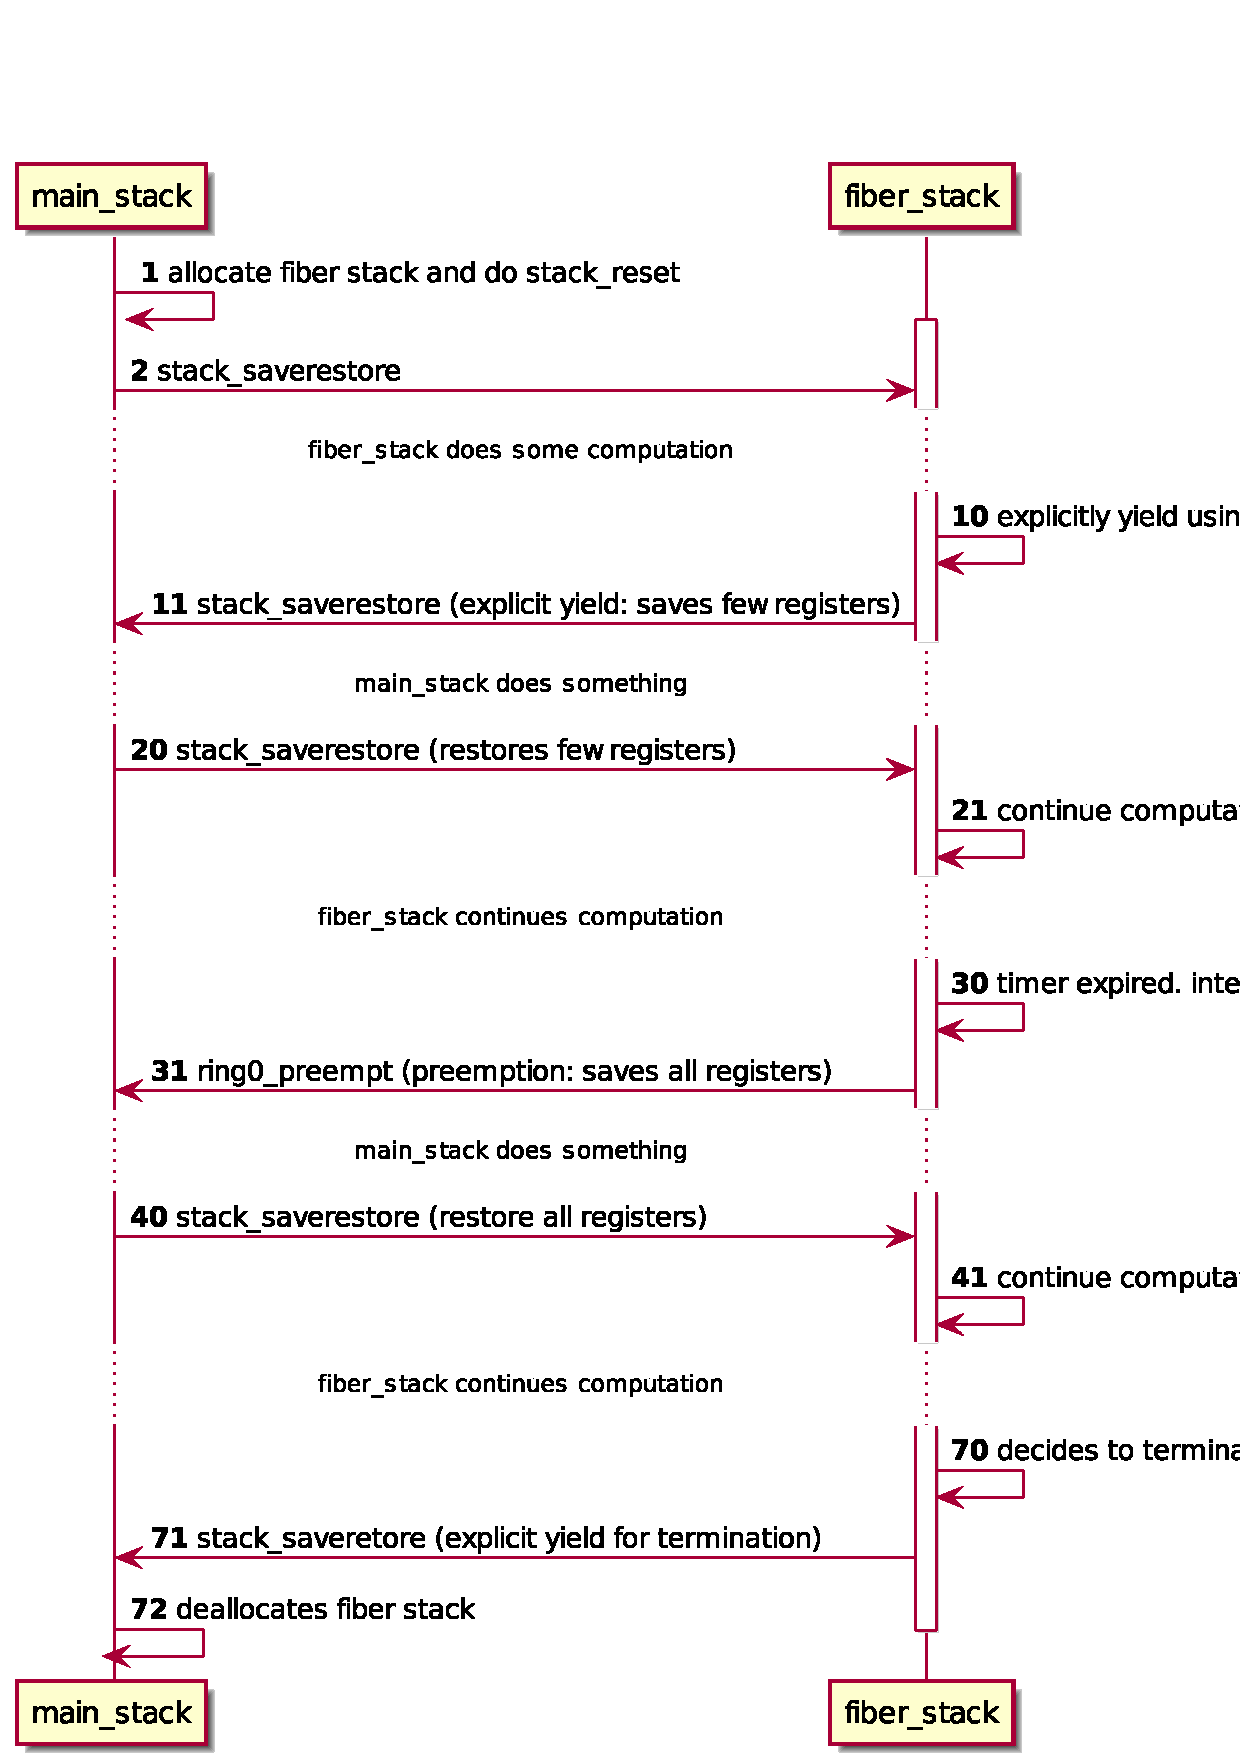
\includegraphics{images/89fb4cb77a4c4ab7b33f32c88bfaccb7b8715408.pdf}

\begin{itemize}
\item
  FPU: eax,ecx, edx, ebx, esp, ebp, esi, edi are all integer registers.

  Let's try to write a simple C functions which add two floats:

\begin{Shaded}
\begin{Highlighting}[]
\DataTypeTok{float} \NormalTok{add(}\DataTypeTok{float} \NormalTok{a, }\DataTypeTok{float} \NormalTok{b)\{}
   \KeywordTok{return} \NormalTok{a+b;}
\NormalTok{\}}
\end{Highlighting}
\end{Shaded}

  Which registers are they going to use, and which instructions?
  integers registers? addl instruction? No! What's the format of floats?
  number is represented as (sign,mantisa,exponent). To know about it,
  please read about IEEE754 floating point representation/basic computer
  architecture course. That's where legacy 8087 FPU comes into picture.

  It has 8 80-bit FPU registers: st(0),st(1), st(2)\ldots{}st(7). ( 1
  bit sign, 64 bit mantissa, 15 bit exponent) sizeof(double)=8. Floating
  point loads and stores will convert this 80-bit representation to 64
  bit representation when it store to memory.. and viceversa. To know
  about FPU registers, please read:
  \href{http://www.cse.iitd.ac.in/~deepak/lab1/intel.pdf}{Vol-1, Chapter
  8}
\item
  MMX/SIMD2: With one instruction, we want to add N pairs in parallel,
  which means we want registers than hold N ints (or N floats).

  x86 has mm0, mm1, mm2.. mm7 (which are SIMD2, ie. N=2 - it holds two
  floats). To know more about MMx registers, please read:
  \href{http://www.cse.iitd.ac.in/~deepak/hohlabs/intel.pdf}{Vol-1
  Chapter 9}
\item
  SSE/SIMD4: It also introduced SIMD4(128 bit registers) xmm registers.
  xmm0, xmm1 \ldots{} xmm7. To know more about xmm registers, please
  read: \href{http://www.cse.iitd.ac.in/~deepak/hohlabs/intel.pdf}{Vol-1
  Chapter 10}
\item
  AVX/SIMD8 Intel also introduced (SIMD8) ymm registers in architectures
  like Sandybridge, Haswell etc. but since our gcl machines doesn't
  support these - we won't discuss it here.
\item
  Overview of preemption handler's control flow:
\end{itemize}

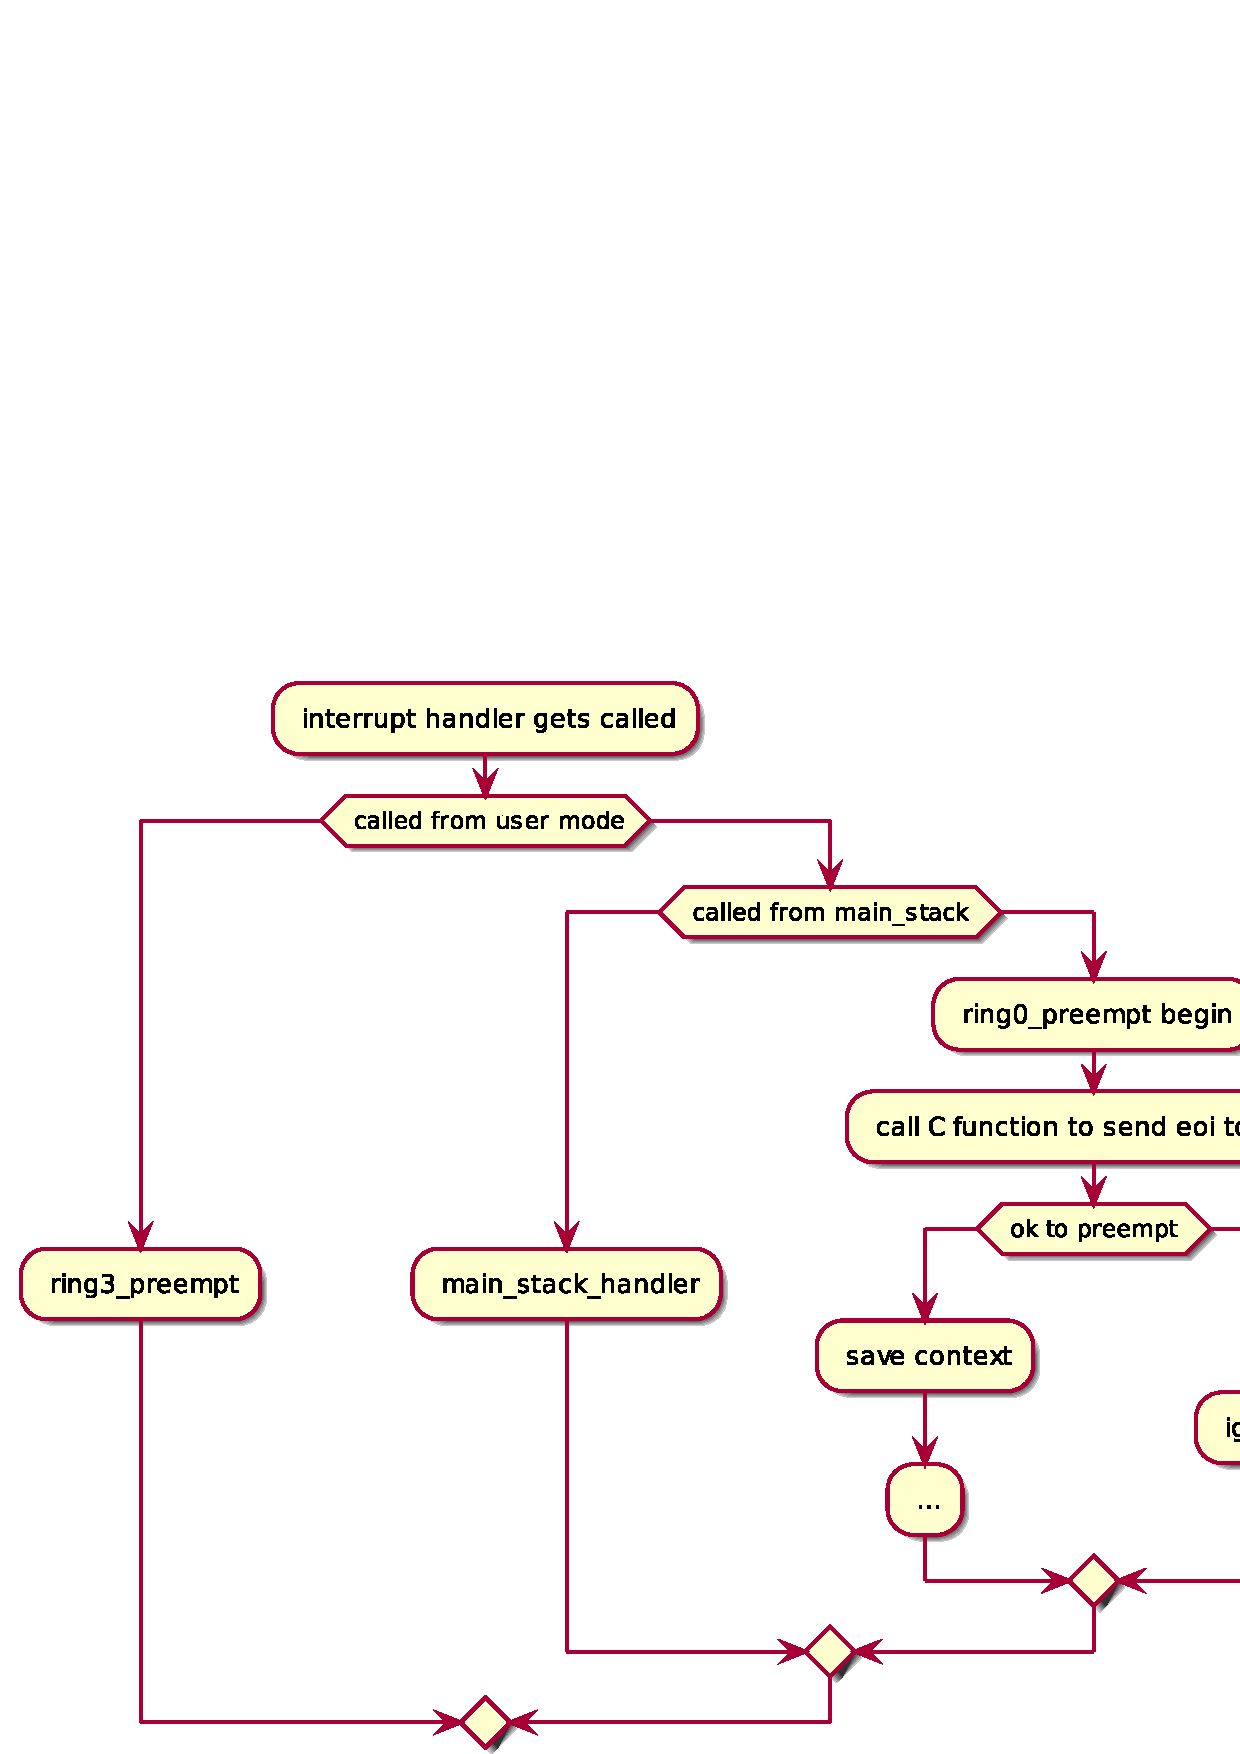
\includegraphics{images/3a92be50adfe22414c4435e355e64cfe7d5cf7e1.pdf}

\subsubsection*{Usage}\label{usage-7}
\addcontentsline{toc}{subsubsection}{Usage}

Read the code - to understand where ring0\_prempt is getting called

\subsubsection*{Define}\label{define-7}
\addcontentsline{toc}{subsubsection}{Define}

You need to define the following structures in labs/preempt.h

\begin{Shaded}
\begin{Highlighting}[]
   \CommentTok{// preempt_t : State for your timer/preemption handler}
   \KeywordTok{struct} \NormalTok{preempt_t\{}
   \NormalTok{\};}
\end{Highlighting}
\end{Shaded}

You also need to define the following functions in labs/preempt.h

\begin{Shaded}
\begin{Highlighting}[]
   \CommentTok{//}
   \CommentTok{// _name: label name}
   \CommentTok{// _f   : C function to be called}
   \CommentTok{//}
   \OtherTok{#  define  _ring0_preempt(_name,_f)            \textbackslash{}}
\end{Highlighting}
\end{Shaded}

You also need to modify labs/fiber.cc and labs/fiber\_schedular.cc to
set the timer and reset the timer

\subsubsection*{Given}\label{given-7}
\addcontentsline{toc}{subsubsection}{Given}

\begin{itemize}
\itemsep1pt\parskip0pt\parsep0pt
\item
  lapic.reset\_timer\_count(N); to generate a timer interrupt after N
  timer ticks (N=0 to stop)

  \begin{itemize}
  \item
    Both the shell\_step\_fiber and shell\_step\_fiber\_sched are passed
    an dev\_lapic\_t object. which has a member function:

\begin{Shaded}
\begin{Highlighting}[]
\NormalTok{reset_timer_count(}\DataTypeTok{int} \NormalTok{count).}
\end{Highlighting}
\end{Shaded}

    LAPIC Timer unit will decrement this count every tick, and when it
    reaches zero, will fire a timer interrupt.

    To know more about LAPIC Timer: please read:
    \href{http://www.cse.iitd.ac.in/~deepak/hohlabs/intel.pdf}{Vol 3A,
    10.5.4.}
  \end{itemize}
\item
  Our kernel does not have any global variables, and our trap handler is
  stateless. So we map our state to \%gs. ie. \%gs:0 will point to
  zeroth byte of core\_t structure. \%gs:1 will point to first byte.. so
  on (Read the code for more info).
\end{itemize}

\subsubsection*{Tip}\label{tip-7}
\addcontentsline{toc}{subsubsection}{Tip}

\begin{itemize}
\item
  Make sure you understand the stack\_saverestore(util/fiber.h) function
  you used in 1.6 and 1.7 parts.
\item
  \%gs: See x86/main.h and x86/except.* on usage of \%gs
\item
  Outline of ring0\_preempt:
\end{itemize}

\begin{Shaded}
\begin{Highlighting}[]

   \OtherTok{#define _ring0_preempt(_name,_f)}

   \NormalTok{_name:}
         \NormalTok{call C function: _f}

         \CommentTok{// begin}
         \KeywordTok{if} \NormalTok{thread is already inside yield,}
           \NormalTok{jmp iret_toring0}

         \NormalTok{save the CPU state to core_t.preempt.foo}
         \KeywordTok{switch} \NormalTok{stack}
         \NormalTok{restore CPU state from core_t.main_stack}
         \CommentTok{// end}

         \NormalTok{jmp iret_toring0}
\end{Highlighting}
\end{Shaded}

\subsubsection*{Turn in}\label{turn-in-7}
\addcontentsline{toc}{subsubsection}{Turn in}

\subsubsection*{Check}\label{check-7}
\addcontentsline{toc}{subsubsection}{Check}

\begin{itemize}
\itemsep1pt\parskip0pt\parsep0pt
\item
  On key press, the status bar shall be updated with `the number of keys
  pressed so far' while the long computation task is running(not after
  it finishes).
\item
  Result of all the three menu items should be same.
\item
  On demand timer ticks: No timer ticks if there're no fibers running.
\end{itemize}

\subsubsection*{Note}\label{note-9}
\addcontentsline{toc}{subsubsection}{Note}

NA

\section{SPSC Queue: Execute task on remote
core}\label{spsc-queue-execute-task-on-remote-core}

\subsubsection*{MergeRequest}\label{mergerequest-8}
\addcontentsline{toc}{subsubsection}{MergeRequest}

I've added few more code in origin/multicore branch. Please merge it
with your master branch

\begin{Shaded}
\begin{Highlighting}[]
    \KeywordTok{user@host}\NormalTok{:~/hohlabs$ git pull}
    \KeywordTok{user@host}\NormalTok{:~/hohlabs$ git merge origin/multicore}
\end{Highlighting}
\end{Shaded}

\subsubsection*{Aim}\label{aim-8}
\addcontentsline{toc}{subsubsection}{Aim}

In this part, we'll learn about multicore programming by implementing a
SPSC queue and use it to send messages between two cores.

\begin{itemize}
\itemsep1pt\parskip0pt\parsep0pt
\item
  I've modified the apps/labs.cc to execute the render() function in
  another core. The output of shell\_render() - renderstate\_t object -
  will be send to core \#1 using the SPSQ queue. And core \#1, will call
  the render() when it receives the renderstate\_t object. Note: this
  means you won't see shell untill you implement SPSC queue correctly.
\item
  You'll have to implement Leslie Lamport's portable lock-free
  single-producer single-consumer bounded buffer algorithm, modified to
  suit the given template
\item
  Size of buffer will always be a power of 2.
\end{itemize}

\subsubsection*{Information}\label{information-8}
\addcontentsline{toc}{subsubsection}{Information}

\begin{itemize}
\itemsep1pt\parskip0pt\parsep0pt
\item
  Leslie Lamport's \href{proving.pdf}{Proving the Correctness of
  Multiprocess Programs}
\item
  gcc atomic intrinsics
\item
  C11/C++11 atomics
\end{itemize}

\subsubsection*{Usage}\label{usage-8}
\addcontentsline{toc}{subsubsection}{Usage}

\begin{itemize}
\itemsep1pt\parskip0pt\parsep0pt
\item
  Please read the code (apps/labs.cc) to see the usage.
\end{itemize}

\subsubsection*{Define}\label{define-8}
\addcontentsline{toc}{subsubsection}{Define}

\begin{itemize}
\itemsep1pt\parskip0pt\parsep0pt
\item
  Shared data structure between producer and consumer
\item
  This data structure is shared between producer and consumer
\item
  We'll reuse this data structure again when we implement user IPC. So
  you shouldn't use any instructions like cli/sti.
\item
  This shared data structure may be accessed from different address
  space. ie. Producer may access this shared data structure with a
  different virtual address than consumer. So you shouldn't use any
  pointers inside this shared data structure.
\end{itemize}

\begin{Shaded}
\begin{Highlighting}[]
\KeywordTok{struct} \NormalTok{channel_t\{}

\NormalTok{\};}
\end{Highlighting}
\end{Shaded}

\begin{itemize}
\itemsep1pt\parskip0pt\parsep0pt
\item
  The producer
\end{itemize}

\begin{Shaded}
\begin{Highlighting}[]

\KeywordTok{struct} \NormalTok{writeport_t\{}


  \CommentTok{//}
  \CommentTok{// Writer}
  \CommentTok{//}


  \CommentTok{// no of entries available to write}
  \NormalTok{size_t write_reservesize();}

  \CommentTok{// Can write 'n' entries?}
  \NormalTok{bool write_canreserve(size_t n);}

  \CommentTok{// Reserve 'n' entries for write}
  \NormalTok{size_t write_reserve(size_t n);}


  \CommentTok{//}
  \CommentTok{// Deleter}
  \CommentTok{//}


  \CommentTok{// No of entires available to delete}
  \NormalTok{size_t delete_reservesize();}


  \CommentTok{// Can delete 'n' entires?}
  \NormalTok{bool delete_canreserve(size_t n);}


  \CommentTok{// Reserve 'n' entires for deletion}
  \NormalTok{size_t delete_reserve(size_t n);}



  \CommentTok{//}
  \CommentTok{// Synchronized operations}
  \CommentTok{//}
  \CommentTok{// Note: Feel free to implement these functions the way you want.}
  \CommentTok{//       You're not allowed to change the function prototype}
  \CommentTok{// PS:   Don't go by the function names.}
  \CommentTok{//}

  \CommentTok{// Read/Write shared memory data structure}
  \DataTypeTok{void} \NormalTok{write_sync(channel_t& ch);}

  \CommentTok{// Read/Write shared memory data structure}
  \DataTypeTok{void} \NormalTok{read_sync(channel_t& ch);}

  \CommentTok{// Update the state, if any.}
  \DataTypeTok{void} \NormalTok{delete_sync();}


\NormalTok{\};}
\end{Highlighting}
\end{Shaded}

\begin{itemize}
\itemsep1pt\parskip0pt\parsep0pt
\item
  Consumer
\end{itemize}

\begin{Shaded}
\begin{Highlighting}[]

\KeywordTok{struct} \NormalTok{readport_t\{}


  \CommentTok{//}
  \CommentTok{// Reader}
  \CommentTok{//}


  \CommentTok{// no of entries available to read}
  \NormalTok{size_t read_reservesize();}

  \CommentTok{// Can Read 'n' entires?}
  \NormalTok{bool read_canreserve(size_t n);}

  \CommentTok{// Reserve 'n' entires to be read}
  \NormalTok{size_t read_reserve(size_t n);}



  \CommentTok{//}
  \CommentTok{// Synchronization operation}
  \CommentTok{//}
  \CommentTok{// Note: Feel free to implement these functions the way you want.}
  \CommentTok{//       You're not allowed to change the function prototype}
  \CommentTok{// PS:   Don't go by the function names.}

  \CommentTok{// Read/write shared memory data structure}
  \DataTypeTok{void} \NormalTok{read_sync(channel_t& ch);}

  \CommentTok{// Read/Write shared memory data structure}
  \DataTypeTok{void} \NormalTok{write_sync(channel_t& ch);}

\NormalTok{\};}
\end{Highlighting}
\end{Shaded}

\subsubsection*{Given}\label{given-8}
\addcontentsline{toc}{subsubsection}{Given}

NA

\subsubsection*{Tip}\label{tip-8}
\addcontentsline{toc}{subsubsection}{Tip}

\begin{itemize}
\itemsep1pt\parskip0pt\parsep0pt
\item
  use \texttt{std::atomic\textless{}T\textgreater{}}
\item
  Note that shell\_update may be called multiple times before
  shell\_step or other functions will be called. If you've made a hack
  on lab 1.4(shell): like if you assumed that shell\_step() will be
  called exactly after shell\_step() and exactly the same number of
  times - it's time to fix your shell.
\end{itemize}

PS: shell\_update() is your keyboard handler, on every key press it will
be called. it's independent of shell\_step()

\subsubsection*{Turn in}\label{turn-in-8}
\addcontentsline{toc}{subsubsection}{Turn in}

\subsubsection*{Check}\label{check-8}
\addcontentsline{toc}{subsubsection}{Check}

\begin{itemize}
\itemsep1pt\parskip0pt\parsep0pt
\item
  Shell will start to work once you implement render() correctly.
\end{itemize}

\subsubsection*{Note}\label{note-10}
\addcontentsline{toc}{subsubsection}{Note}

\section{Ring3}\label{ring3}

\subsubsection*{MergeRequest}\label{mergerequest-9}
\addcontentsline{toc}{subsubsection}{MergeRequest}

I've added few more code in origin/ring3 branch. Please merge it with
your master branch

\begin{Shaded}
\begin{Highlighting}[]
    \KeywordTok{user@host}\NormalTok{:~/hohlabs$ git pull}
    \KeywordTok{user@host}\NormalTok{:~/hohlabs$ git merge origin/ring3}
\end{Highlighting}
\end{Shaded}

\subsubsection*{Aim}\label{aim-9}
\addcontentsline{toc}{subsubsection}{Aim}

In this part, we'll learn about ELF headers, page table handling and
user mode switching while enhancing our kernel to load arbitary user
program and execute it.

\begin{itemize}
\itemsep1pt\parskip0pt\parsep0pt
\item
  You need to implement elf loader:

  \begin{itemize}
  \itemsep1pt\parskip0pt\parsep0pt
  \item
    You shall only support Position Independent Executable.
  \item
    The entire program memory address space specified by the program
    shall be read only. You can safely ignore the flags in ELF and
    override with `WRITE' flags in page table.
  \item
    The entire program memory address space shall fit into a single
    large page.
  \end{itemize}
\item
  The given file is already in memory. You don't need to load the file
  from disk. You only need to:

  \begin{itemize}
  \itemsep1pt\parskip0pt\parsep0pt
  \item
    allocate new memory for the process.
  \item
    copy the contents at right location
  \item
    setup the process's state:

    \begin{itemize}
    \itemsep1pt\parskip0pt\parsep0pt
    \item
      register values
    \item
      page table
    \item
      allocate memory for kernel \textless{}-\textgreater{} process
      communication.
    \item
      setup the emergency stack layout correctly.
    \end{itemize}
  \end{itemize}
\item
  kernel interrupts if occurred when CPU is in ring3, traphandlers are
  executed with esp=main\_stack\_end. So no need to save esp when you
  switch to ring 3.
\end{itemize}

\includegraphics{graphviz-images/35fb0c92f47d3e29205a5e8b6f7f0643059d4b17.pdf}

\begin{itemize}
\itemsep1pt\parskip0pt\parsep0pt
\item
  You need to load the program's page table.
\item
  We'll implement exit system call later. We'll verify correctness by
  looking at qemu's instruction trace.
\item
  Emergency Stack layout:

  \begin{itemize}
  \item
    type of \_start is:

\begin{Shaded}
\begin{Highlighting}[]
  \DataTypeTok{void} \NormalTok{_start(}\DataTypeTok{uint32_t} \NormalTok{rank, }\DataTypeTok{uint32_t} \NormalTok{masterro, }\DataTypeTok{uint32_t} \NormalTok{masterrw, }\DataTypeTok{uint32_t} \NormalTok{sharedrw)}
\end{Highlighting}
\end{Shaded}

    \begin{itemize}
    \itemsep1pt\parskip0pt\parsep0pt
    \item
      masterrw: address of page shared between kernel and user
    \item
      value of rank, masterro, sharedrw shall be zero.
    \end{itemize}
  \item
    Emergency Stack:

    \begin{itemize}
    \itemsep1pt\parskip0pt\parsep0pt
    \item
      0: rank
    \item
      4: masterro
    \item
      8: masterrw
    \item
      12: sharedrw
    \end{itemize}
  \end{itemize}
\end{itemize}

\includegraphics{graphviz-images/f3006b44bfcfbb88aaffa02f09c92c6ec0ebc1e4.pdf}

\begin{itemize}
\itemsep1pt\parskip0pt\parsep0pt
\item
  Page table:

  \begin{itemize}
  \itemsep1pt\parskip0pt\parsep0pt
  \item
    Identity mapped - please make sure pages you tried are identity
    mapped, and use page table only for protection.
  \end{itemize}
\end{itemize}

\subsubsection*{Information}\label{information-9}
\addcontentsline{toc}{subsubsection}{Information}

Please see lecture videos:

\begin{itemize}
\itemsep1pt\parskip0pt\parsep0pt
\item
  \href{}{ELF headers}
\item
  \href{}{Page table}
\item
  \href{}{First user program}
\end{itemize}

\subsubsection*{Usage}\label{usage-9}
\addcontentsline{toc}{subsubsection}{Usage}

\subsubsection*{Define}\label{define-9}
\addcontentsline{toc}{subsubsection}{Define}

\begin{itemize}
\itemsep1pt\parskip0pt\parsep0pt
\item
  load the elf file contents from the range (from,fromsize) and
  initialize the process `proc'
\item
  (from, fromsize) : ELF
\item
  proc : process structure
\item
  pool4M : a simple pool manager.
\end{itemize}

\begin{Shaded}
\begin{Highlighting}[]
\DataTypeTok{static} \KeywordTok{inline} \DataTypeTok{void} \NormalTok{elf_load(addr_t from, size_t fromsize, process_t& proc, bitpool_t& pool4M);}
\end{Highlighting}
\end{Shaded}

\begin{itemize}
\itemsep1pt\parskip0pt\parsep0pt
\item
  restore process's state from proc.

  \begin{itemize}
  \itemsep1pt\parskip0pt\parsep0pt
  \item
    you need to restore all the registers
  \item
    you need to switch to process's page table.
  \item
    switch to user mode.
  \end{itemize}
\item
  This function shall not return. So you don't need to save current
  stack pointer or local variables.
\end{itemize}

\begin{Shaded}
\begin{Highlighting}[]
\DataTypeTok{static} \KeywordTok{inline} \DataTypeTok{void} \NormalTok{ring3_step(preempt_t& preempt, process_t& proc, dev_lapic_t& lapic);}
\end{Highlighting}
\end{Shaded}

\begin{itemize}
\itemsep1pt\parskip0pt\parsep0pt
\item
  This function shall be called after process is preempted.
\end{itemize}

\begin{Shaded}
\begin{Highlighting}[]
\DataTypeTok{static} \KeywordTok{inline} \DataTypeTok{void} \NormalTok{ring3_step_done(process_t& proc, dev_lapic_t& lapic);}
\end{Highlighting}
\end{Shaded}

\subsubsection*{Given}\label{given-9}
\addcontentsline{toc}{subsubsection}{Given}

\begin{itemize}
\itemsep1pt\parskip0pt\parsep0pt
\item
  See util/elf.h and util/ring3.h.
\item
  user app to be executed in ring3 is already implemented for you.
\end{itemize}

\subsubsection*{Tip}\label{tip-9}
\addcontentsline{toc}{subsubsection}{Tip}

\subsubsection*{Turn in}\label{turn-in-9}
\addcontentsline{toc}{subsubsection}{Turn in}

\subsubsection*{Check}\label{check-9}
\addcontentsline{toc}{subsubsection}{Check}

\begin{itemize}
\itemsep1pt\parskip0pt\parsep0pt
\item
  You need to verify user program execution by looking at qemu.log
\end{itemize}

\subsubsection*{Note}\label{note-11}
\addcontentsline{toc}{subsubsection}{Note}

\section{Ring3 Preemption}\label{ring3-preemption}

\subsubsection*{MergeRequest}\label{mergerequest-10}
\addcontentsline{toc}{subsubsection}{MergeRequest}

I've added few more code in origin/ring3 branch. Please merge it with
your master branch

\begin{Shaded}
\begin{Highlighting}[]
        \KeywordTok{user@host}\NormalTok{:~/hohlabs$ git pull}
        \KeywordTok{user@host}\NormalTok{:~/hohlabs$ git merge origin/ring3}
\end{Highlighting}
\end{Shaded}

\subsubsection*{Aim}\label{aim-10}
\addcontentsline{toc}{subsubsection}{Aim}

In this part, we'll learn about preempting user program while enhancing
our kernel to make it responsive to key presses while long computation
task is running in ring3/user mode.

\begin{itemize}
\itemsep1pt\parskip0pt\parsep0pt
\item
  We'll have single kernel stack for the all user processes.
\item
  Note: On timer interrupt, hardware will automatically switch to
  main\_stack. and ring3\_preempt macro will eventually be called.
\item
  You need to write a part of trap handler - ring3\_preempt - which
  should:

  \begin{itemize}
  \itemsep1pt\parskip0pt\parsep0pt
  \item
    save all register state to current running process's state.
  \item
    intializes the kernel stack and registers to well known state and
    jump to core\_loop (done for you).
  \end{itemize}
\item
  Floats and SIMDs(SSE) instructions are allowed in our kernel.
  ring3\_preempt macro shall save FPU/SIMD registers (context) as well
  during the preemption.
\item
  Note: kernel interrupts if occurred when CPU is in ring3, traphandlers
  are executed with esp=main\_stack\_end.
\item
  Note: Please read the lecture videos to understand how hardware
  context switch works
\item
  Note: Basic understanding of x86/except.\{h,cc\} is required - covered
  in detail during part 1.8.
\end{itemize}

\subsubsection*{Information}\label{information-10}
\addcontentsline{toc}{subsubsection}{Information}

Please see following lecture videos: - \href{}{Process context switch}

\begin{itemize}
\itemsep1pt\parskip0pt\parsep0pt
\item
  When ring3\_upcall, ring3\_downcall, ring3\_preempt, ring0\_preempt is
  getting called: The stack layout is:
\end{itemize}

\includegraphics{graphviz-images/4b94c712fc5d8fc832a722cc09de70139197fc2d.pdf}

\subsubsection*{Usage}\label{usage-10}
\addcontentsline{toc}{subsubsection}{Usage}

\subsubsection*{Define}\label{define-10}
\addcontentsline{toc}{subsubsection}{Define}

In labs/ring3\_preempt.h:

\begin{Shaded}
\begin{Highlighting}[]
   \OtherTok{#define _ring3_preempt(_name, _f)}
\end{Highlighting}
\end{Shaded}

\subsubsection*{Given}\label{given-10}
\addcontentsline{toc}{subsubsection}{Given}

NA

\subsubsection*{Tip}\label{tip-10}
\addcontentsline{toc}{subsubsection}{Tip}

NA

\subsubsection*{Turn in}\label{turn-in-10}
\addcontentsline{toc}{subsubsection}{Turn in}

\subsubsection*{Check}\label{check-10}
\addcontentsline{toc}{subsubsection}{Check}

\begin{itemize}
\itemsep1pt\parskip0pt\parsep0pt
\item
  Responsive shell.
\end{itemize}

\subsubsection*{Note}\label{note-12}
\addcontentsline{toc}{subsubsection}{Note}

\section{Upcall/Signals}\label{upcallsignals}

\subsubsection*{MergeRequest}\label{mergerequest-11}
\addcontentsline{toc}{subsubsection}{MergeRequest}

\begin{Shaded}
\begin{Highlighting}[]
    \KeywordTok{user@host}\NormalTok{:~/hohlabs$ git pull}
    \KeywordTok{user@host}\NormalTok{:~/hohlabs$ git merge origin/ring3}
\end{Highlighting}
\end{Shaded}

\subsubsection*{Aim}\label{aim-11}
\addcontentsline{toc}{subsubsection}{Aim}

In this part, we'll learn about upcalls by letting the user process
manage the exceptions(like INT3, page faults etc).

\begin{itemize}
\itemsep1pt\parskip0pt\parsep0pt
\item
  Whenever exception occur, You need to:

  \begin{itemize}
  \itemsep1pt\parskip0pt\parsep0pt
  \item
    allocate emergency stack at the end of the page shared between
    kernel and user
  \item
    setup the emergency stack layout correctly
  \item
    Set the esp to this allocated emergency stack
  \item
    Set the eip to proc.startip+4.
  \item
    all other register values including eflags shall remain unchanged
  \end{itemize}
\item
  user's exception handler is located at \_start+4. ie.
  (proc.startip+4).
\item
  Emergency Stack layout:

  \begin{itemize}
  \item
    type of (\_start+4) is:

\begin{Shaded}
\begin{Highlighting}[]
\DataTypeTok{void} \NormalTok{user_exception(}\DataTypeTok{uint32_t} \NormalTok{rank, }\DataTypeTok{uint32_t} \NormalTok{masterro, }\DataTypeTok{uint32_t} \NormalTok{masterrw, }\DataTypeTok{uint32_t} \NormalTok{sharedrw, }\DataTypeTok{uint32_t} \NormalTok{num, }\DataTypeTok{uint32_t} \NormalTok{errorcode, }\DataTypeTok{uint32_t} \NormalTok{oldesp, }\DataTypeTok{uint32_t} \NormalTok{old_eip, }\DataTypeTok{uint32_t} \NormalTok{cr2)}
\end{Highlighting}
\end{Shaded}

    \begin{itemize}
    \itemsep1pt\parskip0pt\parsep0pt
    \item
      num: Exception number
    \item
      errorcode: errorcode pushed by exception handler, if any.
      otherwise zero.
    \end{itemize}
  \item
    Emergency Stack:

    \begin{itemize}
    \itemsep1pt\parskip0pt\parsep0pt
    \item
      0: rank
    \item
      4: masterro
    \item
      8: masterrw
    \item
      12: sharedrw
    \item
      16: num
    \item
      20: errorcode
    \item
      24: \%old\_esp
    \item
      28: \%old\_eip
    \item
      32: cr2
    \end{itemize}
  \end{itemize}
\end{itemize}

\includegraphics{graphviz-images/d50928bd7002c13646279d8fab8054c249347161.pdf}

\subsubsection*{Information}\label{information-11}
\addcontentsline{toc}{subsubsection}{Information}

\begin{itemize}
\itemsep1pt\parskip0pt\parsep0pt
\item
  When ring3\_upcall, ring3\_downcall, ring3\_preempt, ring0\_preempt is
  getting called: The stack layout is:
\end{itemize}

\includegraphics{graphviz-images/4b94c712fc5d8fc832a722cc09de70139197fc2d.pdf}

\subsubsection*{Usage}\label{usage-11}
\addcontentsline{toc}{subsubsection}{Usage}

\subsubsection*{Define}\label{define-11}
\addcontentsline{toc}{subsubsection}{Define}

In labs/ring3\_upcall.h:

\begin{Shaded}
\begin{Highlighting}[]
   \OtherTok{#define _ring3_upcall(_name, _f)}
\end{Highlighting}
\end{Shaded}

\subsubsection*{Given}\label{given-11}
\addcontentsline{toc}{subsubsection}{Given}

NA

\subsubsection*{Tip}\label{tip-11}
\addcontentsline{toc}{subsubsection}{Tip}

NA

\subsubsection*{Turn in}\label{turn-in-11}
\addcontentsline{toc}{subsubsection}{Turn in}

\subsubsection*{Check}\label{check-11}
\addcontentsline{toc}{subsubsection}{Check}

Generate an int3 or a page fault yourself. and see if it is getting
reported correctly. ie. Match the values in qemu.log and the ones
printed by user\_exception handler.

\subsubsection*{Note}\label{note-13}
\addcontentsline{toc}{subsubsection}{Note}

\section{Downcall/System call}\label{downcallsystem-call}

\subsubsection*{MergeRequest}\label{mergerequest-12}
\addcontentsline{toc}{subsubsection}{MergeRequest}

\begin{Shaded}
\begin{Highlighting}[]
    \KeywordTok{user@host}\NormalTok{:~/hohlabs$ git pull}
    \KeywordTok{user@host}\NormalTok{:~/hohlabs$ git merge origin/ring3}
\end{Highlighting}
\end{Shaded}

\subsubsection*{Aim}\label{aim-12}
\addcontentsline{toc}{subsubsection}{Aim}

In this part, we'll learn about downcalls/system calls by implementing
following system calls: - You need to define the following function:
system\_call();

\begin{enumerate}
\def\labelenumi{\arabic{enumi}.}
\setcounter{enumi}{-1}
\itemsep1pt\parskip0pt\parsep0pt
\item
  \emph{nop}: no-operation/do-nothing

  \begin{itemize}
  \item
    do-nothing
  \item
    System call should \emph{NOT} modify/write to the system call
    memory. (See Tip)

\begin{Shaded}
\begin{Highlighting}[]
\NormalTok{nop()}
\end{Highlighting}
\end{Shaded}
  \end{itemize}
\item
  \emph{done}: done/exit.

  \begin{itemize}
  \item
    mark the process as done(proc-\textgreater{}state=PROC\_DONE).
    process shouldn't be scheduled after this. So make sure, in your
    ring3\_step, you ignore the process if
    proc-\textgreater{}state==PROC\_DONE.

\begin{Shaded}
\begin{Highlighting}[]
\NormalTok{done/exit()}
\end{Highlighting}
\end{Shaded}
  \end{itemize}
\item
  \emph{mmio\_read}: read size bytes from the given address using mmio

  \begin{itemize}
  \item
    call appropriate mmio::read based on the value of size.

\begin{Shaded}
\begin{Highlighting}[]
\NormalTok{mmio_read(size, addr_t) -> value}
\end{Highlighting}
\end{Shaded}
  \end{itemize}
\item
  \emph{mmio\_write}: write size bytes to the given address using mmio

  \begin{itemize}
  \item
    call appropriate mmio::write based on the value of size.

\begin{Shaded}
\begin{Highlighting}[]
\NormalTok{mmio_write(size, addr_t, value)}
\end{Highlighting}
\end{Shaded}
  \end{itemize}
\item
  \emph{pmio\_read}: read size bytes from the given port address using
  pmio

  \begin{itemize}
  \item
    call appropriate io::read based on the value of size.

\begin{Shaded}
\begin{Highlighting}[]
\NormalTok{pmio_read(size, io_t) -> value}
\end{Highlighting}
\end{Shaded}
  \end{itemize}
\item
  \emph{pmio\_write}: write size bytes to the given port address using
  pmio

  \begin{itemize}
  \item
    call appropriate io::write based on the value of size.

\begin{Shaded}
\begin{Highlighting}[]
\NormalTok{pmio_write(size, io_t, value)}
\end{Highlighting}
\end{Shaded}
  \end{itemize}
\item
  \emph{mmu\_swapva}: swap the entry of the process's page table.

  \begin{itemize}
  \item
    make sure both va1 and va2 are in VA\_RANGE.
  \item
    Note: VA\_RANGE is defined as 2GB-3GB.
  \item
    Hint: use proc.mmu.swap(..);
  \item
    Make sure you swap the flags as well. For example: if va1 is not
    mapped into user page, and va2 is mapped, After swap: va1 is mapped
    into user page and va1 is not.

\begin{Shaded}
\begin{Highlighting}[]
\NormalTok{mmu_swapva(va1,va2)}
\end{Highlighting}
\end{Shaded}
  \end{itemize}
\item
  \emph{mmu\_mapmmio}: grants access to the requested page.

  \begin{itemize}
  \item
    maps the corresponding page into user space with (VA=PA)
  \item
    Note: nva should \emph{NOT} be in VA\_RANGE.
  \item
    Note: VA\_RANGE is defined as 2GB-3GB.

\begin{Shaded}
\begin{Highlighting}[]
\NormalTok{mmu_mapmmio(nva)}
\end{Highlighting}
\end{Shaded}
  \end{itemize}
\item
  \emph{pmu\_mappmio}: grants access to the requested io port.

  \begin{itemize}
  \item
    for time being, set iopl flags to 3. ie. proc-\textgreater{}iopl=3.
    and always make sure eflags = (eflags \&
    \textasciitilde{}(3u\textless{}\textless{}12)) \textbar{}
    (proc-\textgreater{}iopl\textless{}\textless{}12);

\begin{Shaded}
\begin{Highlighting}[]
\NormalTok{pmu_mappmio(io_t)}
\end{Highlighting}
\end{Shaded}
  \end{itemize}
\item
  \emph{pool\_alloc}: allocate a large page from pool4M and maps into
  user address space

  \begin{itemize}
  \item
    returns 0, if a large page cannot be allocated from pool4M
  \item
    allocates a large page from the pool4M, and
  \item
    finds an entry in VA\_RANGE which is not mapped into user space,
    maps the page into this unused address in VA\_RANGE with user
    privileges. returns this new va.
  \item
    Note: Newly allocated page is already mapped into kernel address
    space with VA=PA, coz of identity page table(with permissions as
    Kernel only). Please don't change this mapping.
  \item
    Note: VA\_RANGE is defined as 2GB-3GB.
  \item
    Note: unused page in VA\_RANGE is defined as: a page with kernel
    privileges.
  \item
    Note: after this page table is no longer identity mapped. So make
    sure you save and restore kernel's page table.
  \item
    Note: This system call returns either 0 or a va within the range
    VA\_RANGE.

\begin{Shaded}
\begin{Highlighting}[]
\NormalTok{pool_alloc() -> va}
\end{Highlighting}
\end{Shaded}
  \end{itemize}
\end{enumerate}

Note: No need to implement authorization. We haven't implemented support
for capabilities in this kernel yet. We'll implement capabilities in IPC
part only.

User shall pass arguments through begin of page shared between user and
kernel. Memory layout:

\begin{itemize}
\itemsep1pt\parskip0pt\parsep0pt
\item
  0: reserved. must be zero.
\item
  4: Syscall num. Zero indicates No syscall request pending.
\item
  8: Syscall Arg1 / Syscall Ret1.
\item
  12: Syscall Arg2 / Syscall Ret2.
\item
  16: Syscall Arg3 / Syscall Ret3.
\end{itemize}

\includegraphics{graphviz-images/47fc597a5f4ea59d064276c7b792ba3ec05d947f.pdf}

Kernel may execute system call asynchronously by reading the shared
page. User can alternatively force the use of system call execution, by
using INT 0x48.

Note: Make sure In elf\_load() you clears first 64 byte of
proc.masterrw. esp. initialize proc.masterrw{[}0{]} as zero.

\subsubsection*{Information}\label{information-12}
\addcontentsline{toc}{subsubsection}{Information}

NA

\subsubsection*{Usage}\label{usage-12}
\addcontentsline{toc}{subsubsection}{Usage}

\begin{Shaded}
\begin{Highlighting}[]


\DataTypeTok{static} \KeywordTok{inline} \DataTypeTok{void} \NormalTok{xsyscall(}\DataTypeTok{uint32_t}\NormalTok{* systemcallmmio, }\DataTypeTok{uint32_t} \NormalTok{fnum, }\DataTypeTok{uint32_t} \NormalTok{arg1, }\DataTypeTok{uint32_t} \NormalTok{arg2, }\DataTypeTok{uint32_t} \NormalTok{arg3, }\DataTypeTok{uint32_t}\NormalTok{& ret1, }\DataTypeTok{uint32_t}\NormalTok{& ret2, }\DataTypeTok{uint32_t}\NormalTok{& ret3)\{}

  \NormalTok{systemcallmmio[}\DecValTok{2}\NormalTok{]=arg1;}
  \NormalTok{systemcallmmio[}\DecValTok{3}\NormalTok{]=arg2;}
  \NormalTok{systemcallmmio[}\DecValTok{4}\NormalTok{]=arg3;}
  \NormalTok{systemcallmmio[}\DecValTok{1}\NormalTok{]=fnum; }\CommentTok{//write this field at the end.}

  \NormalTok{hoh_debug(}\StringTok{"Shell Before making system call"}\NormalTok{);}
  \NormalTok{asm }\DataTypeTok{volatile}\NormalTok{(}\StringTok{"int $0x48"}\NormalTok{:::}\StringTok{"memory"}\NormalTok{);}
  \NormalTok{hoh_debug(}\StringTok{"Shell After making system call"}\NormalTok{);}

  \NormalTok{hoh_assert(systemcallmmio[}\DecValTok{1}\NormalTok{]==}\DecValTok{0}\NormalTok{,}\StringTok{"XXX"}\NormalTok{);}
  \NormalTok{ret1=systemcallmmio[}\DecValTok{2}\NormalTok{];}
  \NormalTok{ret2=systemcallmmio[}\DecValTok{3}\NormalTok{];}
  \NormalTok{ret3=systemcallmmio[}\DecValTok{4}\NormalTok{];}

  \NormalTok{hoh_debug(}\StringTok{"Syscall ret: "}\NormalTok{<<ret1<<}\StringTok{","}\NormalTok{<<ret2<<}\StringTok{","}\NormalTok{<<ret3);}

\NormalTok{\}}




  \CommentTok{// call test_systemcall by:}

  \CommentTok{//swapva}
  \DataTypeTok{uint32_t} \NormalTok{ret1;}
  \DataTypeTok{uint32_t} \NormalTok{ret2;}
  \DataTypeTok{uint32_t} \NormalTok{ret3;}
  \NormalTok{xsyscall(core.syscallmmio, }\BaseNTok{0x6}\NormalTok{, xxx, yyy, }\DecValTok{0}\NormalTok{, ret1, ret2, ret3);}


  \CommentTok{//pool_alloc}
  \DataTypeTok{uint32_t} \NormalTok{ret1;}
  \DataTypeTok{uint32_t} \NormalTok{ret2;}
  \DataTypeTok{uint32_t} \NormalTok{ret3;}
  \NormalTok{xsyscall(systemcallmmio, }\BaseNTok{0x9}\NormalTok{, }\DecValTok{0}\NormalTok{,}\DecValTok{0}\NormalTok{,}\DecValTok{0}\NormalTok{, ret1,ret2,ret3);}
  \NormalTok{hoh_debug(}\StringTok{"Allocated at: "}\NormalTok{<<ret1);}

\end{Highlighting}
\end{Shaded}

\subsubsection*{Define}\label{define-12}
\addcontentsline{toc}{subsubsection}{Define}

\subsubsection*{Given}\label{given-12}
\addcontentsline{toc}{subsubsection}{Given}

NA

\subsubsection*{Tip}\label{tip-12}
\addcontentsline{toc}{subsubsection}{Tip}

\begin{Shaded}
\begin{Highlighting}[]
  \DataTypeTok{uint32_t}\NormalTok{* systemcall_mmio = cast<}\DataTypeTok{uint32_t}\NormalTok{*>(proc.masterrw);}
  \DataTypeTok{uint32_t} \NormalTok{fnum =systemcall_mmio[}\DecValTok{1}\NormalTok{];  }\CommentTok{//read fnum first.}

  \KeywordTok{if}\NormalTok{(fnum==}\DecValTok{0}\NormalTok{)\{ }\CommentTok{//make sure you check fnum.}
    \KeywordTok{return}\NormalTok{;}
  \NormalTok{\}}

  \DataTypeTok{uint32_t} \NormalTok{farg1=systemcall_mmio[}\DecValTok{2}\NormalTok{];}
  \DataTypeTok{uint32_t} \NormalTok{farg2=systemcall_mmio[}\DecValTok{3}\NormalTok{];}
  \DataTypeTok{uint32_t} \NormalTok{farg3=systemcall_mmio[}\DecValTok{4}\NormalTok{];}

  \DataTypeTok{uint32_t} \NormalTok{fret1=}\DecValTok{0}\NormalTok{;}
  \DataTypeTok{uint32_t} \NormalTok{fret2=}\DecValTok{0}\NormalTok{;}
  \DataTypeTok{uint32_t} \NormalTok{fret3=}\DecValTok{0}\NormalTok{;}

  \KeywordTok{switch}\NormalTok{(fnum)\{}
  \KeywordTok{case} \DecValTok{0}\NormalTok{: \{}
          \NormalTok{\}}\KeywordTok{break}\NormalTok{;}
  \KeywordTok{case} \DecValTok{1}\NormalTok{: \{}
          \NormalTok{\}}\KeywordTok{break}\NormalTok{;}
  \KeywordTok{case} \DecValTok{2}\NormalTok{: \{}
          \NormalTok{\}}\KeywordTok{break}\NormalTok{;}
  \NormalTok{\}}


  \KeywordTok{if}\NormalTok{(fnum!=}\DecValTok{0}\NormalTok{)\{}
    \CommentTok{// do not modify the arguments if fnum is zero.}
    \NormalTok{systemcall_mmio[}\DecValTok{2}\NormalTok{]=fret1;}
    \NormalTok{systemcall_mmio[}\DecValTok{3}\NormalTok{]=fret2;}
    \NormalTok{systemcall_mmio[}\DecValTok{4}\NormalTok{]=fret3;}
    \NormalTok{systemcall_mmio[}\DecValTok{1}\NormalTok{]=}\DecValTok{0}\NormalTok{; }\CommentTok{//modify this last.}
  \NormalTok{\}}


\end{Highlighting}
\end{Shaded}

\subsubsection*{Turn in}\label{turn-in-12}
\addcontentsline{toc}{subsubsection}{Turn in}

\begin{itemize}
\itemsep1pt\parskip0pt\parsep0pt
\item
  Implement the given 10 system calls.
\item
  Write test cases for these 10 system calls by modifying ring3/app1(We
  won't check your test cases ie. No marks for test cases).
\end{itemize}

\subsubsection*{Check}\label{check-12}
\addcontentsline{toc}{subsubsection}{Check}

\subsubsection*{Note}\label{note-14}
\addcontentsline{toc}{subsubsection}{Note}

\section{App: Virtual Memory}\label{app-virtual-memory}

\subsubsection*{MergeRequest}\label{mergerequest-13}
\addcontentsline{toc}{subsubsection}{MergeRequest}

\begin{Shaded}
\begin{Highlighting}[]
    \KeywordTok{user@host}\NormalTok{:~/hohlabs$ git pull}
    \KeywordTok{user@host}\NormalTok{:~/hohlabs$ git merge origin/ring3}
\end{Highlighting}
\end{Shaded}

\subsubsection*{Aim}\label{aim-13}
\addcontentsline{toc}{subsubsection}{Aim}

In this part, we'll learn about virtual memory by emulating an array of
\(N_v\) virtual pages using \(N_p\) physical pages.

\begin{itemize}
\item
  \textbf{Note: There is a change : \(N_v=16\) and \(N_p=4\) instead of
  \(N_v=16\) and \(N_p=8\). Ie. you need to emulate 16 page array using
  4 physical pages. not 8}
\item
  Please read lecture videos on demand paging and page replacement
  policy.
\item
  You need to emulate an array of size \(N_v\) pages, say varray.
  Starting address of varray shall be 2GB ie.
  2u\textless{}\textless{}30.
\item
  \(N_v=16\) and \(N_p=4\)
\end{itemize}

\includegraphics{graphviz-images/2623b6fa1d58130a3904de5d38846fcc56312f9d.pdf}

\begin{itemize}
\itemsep1pt\parskip0pt\parsep0pt
\item
  by using exactly \(N_p\) physical pages.
\end{itemize}

\includegraphics{graphviz-images/a0f1bdeb6728d1f45ef7706fb8ab2cf34b03ad49.pdf}

\begin{itemize}
\itemsep1pt\parskip0pt\parsep0pt
\item
  Note: Before allocating these \(N_p\) physical pages, none of elements
  in varray is mapped to user space.
\end{itemize}

\includegraphics{graphviz-images/925fb07dd8a75351299f096096fd68d723c5a480.pdf}

\begin{itemize}
\itemsep1pt\parskip0pt\parsep0pt
\item
  You shall use pool\_alloc system call to allocate a page. You shall
  make exactly N pool\_alloc system calls in your app. Note: pool\_alloc
  system call will always return value within VA\_RANGE. Note: When you
  allocate pages, there is no guarantee that pool\_alloc will return
  them in continous order.
\end{itemize}

\includegraphics{graphviz-images/afbaf87825d4f41b0369cc3d97ea36d4719d0d00.pdf}

\begin{itemize}
\itemsep1pt\parskip0pt\parsep0pt
\item
  You need to swap the page table entries from user mode using:
  mmu\_swapva system call. Note: mmu\_swapva will only swap if the
  arguments are within VA\_RANGE. For example, a valid mapping could be:
\end{itemize}

\includegraphics{graphviz-images/d0b0d4aa89a691fbd2ceed7a05160c25c93500f4.pdf}

\begin{itemize}
\itemsep1pt\parskip0pt\parsep0pt
\item
  You need to test your emulation of this virtual array, varray, by:

  \begin{enumerate}
  \def\labelenumi{\arabic{enumi}.}
  \itemsep1pt\parskip0pt\parsep0pt
  \item
    storing a 3D matrix of type \emph{const
    uint32\_t{[}8{]}{[}8{]}{[}8{]}} into this varray.

    \begin{itemize}
    \item
      You need to define a function to\_index which will map this 3D
      array into varray. ie

\begin{Shaded}
\begin{Highlighting}[]
\CommentTok{//access x,y,z of this 3D array by:}
\NormalTok{varray[to_index(x,y,z)]=f(x,y,z);}
\CommentTok{//or:}
\NormalTok{hoh_assert(varray[to_index(x,y,z)] == f(x,y,z),}\StringTok{" Bug"}\NormalTok{);}
\end{Highlighting}
\end{Shaded}
    \item
      You can map this matrix into any order - not necessarily be
      row-major order.
    \item
      You need to find a mapping `to\_index' that will minimize the
      number of page faults and cache misses.
    \end{itemize}
  \item
    Write a function, `for\_each', which will:

    \begin{itemize}
    \itemsep1pt\parskip0pt\parsep0pt
    \item
      traverse all the elements in this 3D array in some order(strided
      by 32),
    \item
      and print the sum of each element's neighbourhood defined by
      chebyshev distance of \(d=2^6\). See: sum\_neighbours or
      weightedsum\_neigbours in the usage.
    \item
      Note: For each point, sum\_neighbours computes sum of elements in
      its neighbourhood within a Chebyshev distance of \(d=2^6\). (See
      usage).
    \item
      You can traverse the matrix in any order - not necessarily be
      row-major.
    \item
      You need to find a traversal `for\_each' that will will minimize
      the number of page faults and cache misses. ```c
    \end{itemize}
  \end{enumerate}
\end{itemize}

for(uint32\_t x = 0; x\textless{}256; x+=32)\{ for(uint32\_t y = 0;
y\textless{}256; y+=32)\{ for(uint32\_t z = 0; z\textless{}256; z+=32)\{
sum\_neighbours(x,y,z,f\_lut); \} \} \}

``` 3. You need to implement page replacement policy. You need to find a
page replacement policy that will minimize the number of page faults and
cache misses.

\begin{itemize}
\itemsep1pt\parskip0pt\parsep0pt
\item
  Note: Both sum\_neighbours and weightedsum\_neighbours traverse its
  neighbourhood defined by chebyshev distance of \(d=2^6\). Make sure
  you optimize all the three - to\_index, for\_each and page replacement
  policy based on this behaviour.
\item
  You also need to print the number of page fault occurred in your app.
\item
  You're required to implement the code under ring3/app1 directory.
\end{itemize}

Motivation for the application:

\begin{itemize}
\item
  Let's say we've a long computation function

\begin{Shaded}
\begin{Highlighting}[]
  \DataTypeTok{uint32_t} \NormalTok{f(}\DataTypeTok{uint8_t} \NormalTok{x, }\DataTypeTok{uint8_t} \NormalTok{y, }\DataTypeTok{uint8_t} \NormalTok{z);}
\end{Highlighting}
\end{Shaded}
\item
  Usage: Assume we want to call sum\_neighbours and
  weightedsum\_neigbours for each \(x,y,z \in [0..255]\) (See usage)
\item
  To reduce invocation of this function each time we need it. We
  precompute `f' for all the possible inputs and store it in a lookup
  table/array. ie.

\begin{Shaded}
\begin{Highlighting}[]
\KeywordTok{for}\NormalTok{(x=}\DecValTok{0}\NormalTok{;x<=}\DecValTok{255}\NormalTok{;x++)\{}
 \KeywordTok{for}\NormalTok{(y=}\DecValTok{0}\NormalTok{;y<=}\DecValTok{255}\NormalTok{;y++)\{}
  \KeywordTok{for}\NormalTok{(z=}\DecValTok{0}\NormalTok{;z<=}\DecValTok{255}\NormalTok{;z++)\{}
    \NormalTok{varray[to_index(x,y,z)] = f(x,y,z);}
  \NormalTok{\}}
 \NormalTok{\}}
\NormalTok{\}}

\CommentTok{//then, we can replace f with f2 where}
\DataTypeTok{uint32_t} \NormalTok{f2(}\DataTypeTok{uint8_t} \NormalTok{x,}\DataTypeTok{uint8_t} \NormalTok{y,}\DataTypeTok{uint8_t} \NormalTok{z)\{}
  \KeywordTok{return} \NormalTok{varray[to_index(x,y,z)];}
\NormalTok{\}}
\end{Highlighting}
\end{Shaded}
\item
  To memoize the entire function, we require
  \(2^8 * 2^8 * 2^8 * sizeof(uint32_t) = 64MB\) ie. 16 large pages.
\item
  But we have only 4 pages. ie. You can only allocate 4 large pages(call
  pool\_alloc system call 4 times).
\item
  To get f2 working, without any modifications: We will emulate the
  array `varray' of 16 larges pages within VA\_RANGE.

\begin{Shaded}
\begin{Highlighting}[]
\NormalTok{addr_t varray = addr_t(}\DecValTok{2}\NormalTok{<<}\DecValTok{30}\NormalTok{); }\CommentTok{//2GB}
\end{Highlighting}
\end{Shaded}
\item
  We allocate 4 pages, make sure they're mapped into this array and
  intializes the value. If the allocated page is not mapped within
  {[}varray,varray + 16*LARGE\_PAGE\_SIZE) then: use mmu\_swap system
  call to swap with an unmapped page. (Note: To do this you need to
  maintain already mapped pages. (use a bit for each of 16 pages to mark
  if they're being mapped or not)
\item
  When f2 tries to access varray: if the page is \emph{not} mapped,
  hardware will generate a page fault.
\item
  On page-fault: We will swap this page with already initialized page.
  We will use per-process page replacement policy. And we'll
  reinitialize the page data.
\item
  You also need to print the number of page fault occurred in the
  system.
\item
  Demo tip: What should be to\_index(x,y,z) so that it will minimize
  number of page-faults
\item
  Demo tip: We need to call f2(x,y,z) for all possible x,y and z. What
  should be the order in which we should call f(x,y,z) so that it will
  minimize number of page-faults
\item
  Demo tip: What should be to\_index(x,y,z) so that it will minimize
  number of cache-line misses and tlb misses
\item
  Demo tip: We need to call f2(x,y,z) for all possible x,y and z. What
  should be the order in which we should call f(x,y,z) so that it will
  minimize number of cache-line misses and tlb misses
\end{itemize}

Note: Please don't publish the code even after your demo is done(Code is
part of my PhD work).

\subsubsection*{Information}\label{information-13}
\addcontentsline{toc}{subsubsection}{Information}

\subsubsection*{Usage}\label{usage-13}
\addcontentsline{toc}{subsubsection}{Usage}

\begin{Shaded}
\begin{Highlighting}[]
        \CommentTok{//}
        \CommentTok{// Call sum_neighbours for each x<-[0..255], y<-[0..255], z<-[0..255]}
        \CommentTok{//}
        \CommentTok{// You're allowed to change this implementation: }
        \CommentTok{// Note: d is defined to be 2^6. and cannot be changed}
        \DataTypeTok{uint32_t} \NormalTok{sum_neighbours(}\DataTypeTok{uint8_t} \NormalTok{x, }\DataTypeTok{uint8_t} \NormalTok{y, }\DataTypeTok{uint8_t} \NormalTok{z)\{}
           \CommentTok{//computes sum of all the elements in the list defined by }
           \CommentTok{//       [f(x+i,y+j,z+k) | i<-[-d, -(d-1),...,-1,0,1,...,(d-1),d], }
           \CommentTok{//                         j<-[-d, -(d-1),...,-1,0,1,...,(d-1),d], }
           \CommentTok{//                         k<-[-d, -(d-1),...,-1,0,1,...,(d-1),d]]}
           \CommentTok{//ie.  Note d=2^6}
           \NormalTok{size_t sum=}\DecValTok{0}\NormalTok{;}
            \KeywordTok{for}\NormalTok{(}\DataTypeTok{int} \NormalTok{i=-d; i<d; i++)\{}
              \KeywordTok{for}\NormalTok{(}\DataTypeTok{int} \NormalTok{j=-d; j<d; j++)\{}
                 \KeywordTok{for}\NormalTok{(}\DataTypeTok{int} \NormalTok{k=-d; k<d; k++)\{}
                   \NormalTok{sum += f2(x+i, y+j, z+k);}
                 \NormalTok{\}}
              \NormalTok{\}}
            \NormalTok{\}}
        \NormalTok{\}}

        \CommentTok{//}
        \CommentTok{// Call weightedsum_neighbours for each x<-[0..255], y<-[0..255], z<-[0..255]}
        \CommentTok{//}
        \CommentTok{// You're allowed to change this implementation: }
        \CommentTok{// Note: d is defined to be 2^6. and cannot be changed}
        \DataTypeTok{uint32_t} \NormalTok{weightedsum_neighbours(}\DataTypeTok{uint8_t} \NormalTok{x, }\DataTypeTok{uint8_t} \NormalTok{y, }\DataTypeTok{uint8_t} \NormalTok{z)\{}
           \CommentTok{//computes sum of all the elements in the list defined by }
           \CommentTok{//       [f(x+i,y+j,z+k) | i<-[-d, -(d-1),...,-1,0,1,...,(d-1),d], }
           \CommentTok{//                         j<-[-d, -(d-1),...,-1,0,1,...,(d-1),d], }
           \CommentTok{//                         k<-[-d, -(d-1),...,-1,0,1,...,(d-1),d]]}
           \CommentTok{//ie.  Note d=2^6}
           \NormalTok{size_t sum=}\DecValTok{0}\NormalTok{;}
            \KeywordTok{for}\NormalTok{(}\DataTypeTok{int} \NormalTok{i=-d; i<d; i++)\{}
              \KeywordTok{for}\NormalTok{(}\DataTypeTok{int} \NormalTok{j=-d; j<d; j++)\{}
                 \KeywordTok{for}\NormalTok{(}\DataTypeTok{int} \NormalTok{k=-d; k<d; k++)\{}
                   \NormalTok{sum += w(i,j,k,d) * f2(x+i, y+j, z+k);}
                 \NormalTok{\}}
              \NormalTok{\}}
            \NormalTok{\}}
        \NormalTok{\}}

        \CommentTok{//}
        \CommentTok{// Call another traversal for each x<-[0..255], y<-[0..255], z<-[0..255]}
        \CommentTok{//}
        \DataTypeTok{void} \NormalTok{for_aach()\{}
          \KeywordTok{for} \NormalTok{each element in 3D array: }
             \NormalTok{print sum_neighbours(element);}
        \NormalTok{\}}
\end{Highlighting}
\end{Shaded}

Notation: {[}f(x) \textbar{} x\textless{}-{[}1..10{]}{]} as: list of all
f(x) \emph{such that} x \(\in\) {[}1..10{]}

Notation: Read `\textbar{}' as \emph{such that}. Read `\textless{}-' as
\(\in\).

\subsubsection*{Define}\label{define-13}
\addcontentsline{toc}{subsubsection}{Define}

\subsubsection*{Given}\label{given-13}
\addcontentsline{toc}{subsubsection}{Given}

\subsubsection*{Tip}\label{tip-13}
\addcontentsline{toc}{subsubsection}{Tip}

\subsubsection*{Turn in}\label{turn-in-13}
\addcontentsline{toc}{subsubsection}{Turn in}

\subsubsection*{Check}\label{check-13}
\addcontentsline{toc}{subsubsection}{Check}

\begin{itemize}
\itemsep1pt\parskip0pt\parsep0pt
\item
  for all x,y,z: hoh\_assert(f2(x,y,z) == f(x,y,z), ``XXX'');
\item
  Number of pages allocated shall be 4.
\end{itemize}

\subsubsection*{Note}\label{note-15}
\addcontentsline{toc}{subsubsection}{Note}

\section*{App: Shell in user mode}\label{app-shell-in-user-mode}
\addcontentsline{toc}{section}{App: Shell in user mode}

Hello! Alice here!

Congrats on making it so far! It's been a pleasure working with you.

Hope you enjoyed it as well!

Let's try to summarize the plot:

\begin{itemize}
\itemsep1pt\parskip0pt\parsep0pt
\item
  You wrote a shell in kernel mode.
\item
  Then I split the shell into two and rendered the UI on another core.
\item
  Now I've moved your shell into user mode.
\item
  And then I'll split the user shell into two and render the UI on
  another process.
\end{itemize}

In short: - You've implemented kernel coroutines, kernel threads and a
kernel thread scheduler. And implmented a kernel application - shell. -
You also have implemented user coroutines, user threads and a user
thread schedular. And implemented a user application - shell.

\begin{center}\rule{0.5\linewidth}{\linethickness}\end{center}

\emph{Shell is already done for you!} Your shell which you implemented
in part 1.4 is already moved to user mode as an application. So the role
has been revereed - whatever you've done till parts 1.9 are now in user
mode. And parts 1.10 - parts 1.13 are in kernel.

\begin{center}\rule{0.5\linewidth}{\linethickness}\end{center}

\subsubsection*{MergeRequest}\label{mergerequest-14}
\addcontentsline{toc}{subsubsection}{MergeRequest}

\begin{Shaded}
\begin{Highlighting}[]
    \KeywordTok{user@host}\NormalTok{:~/hohlabs$ git pull}
    \KeywordTok{user@host}\NormalTok{:~/hohlabs$ git merge origin/ring3_shell}
\end{Highlighting}
\end{Shaded}

\subsubsection*{Aim}\label{aim-14}
\addcontentsline{toc}{subsubsection}{Aim}

Get User shell working

\begin{center}\rule{0.5\linewidth}{\linethickness}\end{center}

\textbf{Please don't make the source code public even after you finish
this course} - The code you been working on is part of my PhD. Give me
few months - Once we publish our paper, we'll release the entire code
under AGPL3 licence(Current LICENSE doesn't allow the code). Till then
please don't make the publish.

Btw: alice at hohlabs dot in is a real id, and will be active soon.

Wanted to do BTP/MTP/PhD with Sorav Bansal? Send your resume to sbansal
at cse.

\begin{center}\rule{0.5\linewidth}{\linethickness}\end{center}

\begin{center}\rule{0.5\linewidth}{\linethickness}\end{center}

\emph{End of lab one}

\begin{verbatim}
Please make sure you submit the feedback form
--
Regards,
Alice H
Hoh labs
\end{verbatim}

\begin{center}\rule{0.5\linewidth}{\linethickness}\end{center}

\chapter{Applications}\label{applications}

\subsubsection*{Overview}\label{overview-1}
\addcontentsline{toc}{subsubsection}{Overview}

In this lab, we'll use the components we implemented in previous lab to
make a fully functional kernel.

We'll test our kernel by having two applications:

\begin{enumerate}
\def\labelenumi{\arabic{enumi}.}
\itemsep1pt\parskip0pt\parsep0pt
\item
  File system in RAM
\item
  Virtual Memory
\end{enumerate}

\begin{itemize}
\itemsep1pt\parskip0pt\parsep0pt
\item
  Evaluation:

  \begin{itemize}
  \item
    Code component:

    \begin{itemize}
    \itemsep1pt\parskip0pt\parsep0pt
    \item
      \emph{NOTHING : 0 } Not working
    \item
      \emph{PARTIAL : 1 } Partial/buggy - TA is able to find atleast one
      bug in your code
    \item
      \emph{TYPO : 1.5} Code is not clean
    \item
      \emph{CORRECT : 2 } Working code
    \end{itemize}
  \item
    Viva component:

    \begin{itemize}
    \itemsep1pt\parskip0pt\parsep0pt
    \item
      \emph{FLAGGED : 0 } Can not explain his/her own code
    \item
      \emph{JUST\_IMPLEMENTED : 1 } can explain his/her own code but
      can't explain Alice's code
    \item
      \emph{KNOWS\_WHY : 2 } can explain his/her own code + Alice's code
    \end{itemize}
  \item
    Marks for each part is computed by following equation:
    \[ Marks = (W_d * D + W_v * V) \]
  \item
    For 2.1-2.4: \[ W_d = 0.80 \] and \[ W_v = 0.20 \]
  \end{itemize}
\end{itemize}

\section{Shell in Ring 3 : User level
Schedular}\label{shell-in-ring-3-user-level-schedular}

\subsubsection*{MergeRequest}\label{mergerequest-15}
\addcontentsline{toc}{subsubsection}{MergeRequest}

\subsubsection*{Aim}\label{aim-15}
\addcontentsline{toc}{subsubsection}{Aim}

\subsubsection*{Information}\label{information-14}
\addcontentsline{toc}{subsubsection}{Information}

\subsubsection*{Usage}\label{usage-14}
\addcontentsline{toc}{subsubsection}{Usage}

\subsubsection*{Define}\label{define-14}
\addcontentsline{toc}{subsubsection}{Define}

\subsubsection*{Given}\label{given-14}
\addcontentsline{toc}{subsubsection}{Given}

\subsubsection*{Tip}\label{tip-14}
\addcontentsline{toc}{subsubsection}{Tip}

\subsubsection*{Turn in}\label{turn-in-14}
\addcontentsline{toc}{subsubsection}{Turn in}

\subsubsection*{Check}\label{check-14}
\addcontentsline{toc}{subsubsection}{Check}

\subsubsection*{Note}\label{note-16}
\addcontentsline{toc}{subsubsection}{Note}

\section{User IPC: send\_message}\label{user-ipc-sendux5fmessage}

\subsubsection*{MergeRequest}\label{mergerequest-16}
\addcontentsline{toc}{subsubsection}{MergeRequest}

\subsubsection*{Aim}\label{aim-16}
\addcontentsline{toc}{subsubsection}{Aim}

\subsubsection*{Information}\label{information-15}
\addcontentsline{toc}{subsubsection}{Information}

\subsubsection*{Usage}\label{usage-15}
\addcontentsline{toc}{subsubsection}{Usage}

\subsubsection*{Define}\label{define-15}
\addcontentsline{toc}{subsubsection}{Define}

\subsubsection*{Given}\label{given-15}
\addcontentsline{toc}{subsubsection}{Given}

\subsubsection*{Tip}\label{tip-15}
\addcontentsline{toc}{subsubsection}{Tip}

\subsubsection*{Turn in}\label{turn-in-15}
\addcontentsline{toc}{subsubsection}{Turn in}

\subsubsection*{Check}\label{check-15}
\addcontentsline{toc}{subsubsection}{Check}

\subsubsection*{Note}\label{note-17}
\addcontentsline{toc}{subsubsection}{Note}

\section{File system server in user
mode}\label{file-system-server-in-user-mode}

\subsubsection*{MergeRequest}\label{mergerequest-17}
\addcontentsline{toc}{subsubsection}{MergeRequest}

\subsubsection*{Aim}\label{aim-17}
\addcontentsline{toc}{subsubsection}{Aim}

\subsubsection*{Information}\label{information-16}
\addcontentsline{toc}{subsubsection}{Information}

\subsubsection*{Usage}\label{usage-16}
\addcontentsline{toc}{subsubsection}{Usage}

\subsubsection*{Define}\label{define-16}
\addcontentsline{toc}{subsubsection}{Define}

\subsubsection*{Given}\label{given-16}
\addcontentsline{toc}{subsubsection}{Given}

\subsubsection*{Tip}\label{tip-16}
\addcontentsline{toc}{subsubsection}{Tip}

\subsubsection*{Turn in}\label{turn-in-16}
\addcontentsline{toc}{subsubsection}{Turn in}

\subsubsection*{Check}\label{check-16}
\addcontentsline{toc}{subsubsection}{Check}

\subsubsection*{Note}\label{note-18}
\addcontentsline{toc}{subsubsection}{Note}

\section{Virtual memory in user mode}\label{virtual-memory-in-user-mode}

\subsubsection*{MergeRequest}\label{mergerequest-18}
\addcontentsline{toc}{subsubsection}{MergeRequest}

\subsubsection*{Aim}\label{aim-18}
\addcontentsline{toc}{subsubsection}{Aim}

\subsubsection*{Information}\label{information-17}
\addcontentsline{toc}{subsubsection}{Information}

\subsubsection*{Usage}\label{usage-17}
\addcontentsline{toc}{subsubsection}{Usage}

\subsubsection*{Define}\label{define-17}
\addcontentsline{toc}{subsubsection}{Define}

\subsubsection*{Given}\label{given-17}
\addcontentsline{toc}{subsubsection}{Given}

\subsubsection*{Tip}\label{tip-17}
\addcontentsline{toc}{subsubsection}{Tip}

\subsubsection*{Turn in}\label{turn-in-17}
\addcontentsline{toc}{subsubsection}{Turn in}

\subsubsection*{Check}\label{check-17}
\addcontentsline{toc}{subsubsection}{Check}

\subsubsection*{Note}\label{note-19}
\addcontentsline{toc}{subsubsection}{Note}

\begin{center}\rule{0.5\linewidth}{\linethickness}\end{center}

\emph{End of lab two}

\begin{verbatim}
Please make sure you submit the feedback form
--
Regards,
Alice H
Hoh labs
\end{verbatim}

\begin{center}\rule{0.5\linewidth}{\linethickness}\end{center}

\chapter{HoH Kernel}\label{hoh-kernel}

\subsubsection*{Overview}\label{overview-2}
\addcontentsline{toc}{subsubsection}{Overview}

\begin{itemize}
\itemsep1pt\parskip0pt\parsep0pt
\item
  .
\item
  .
\end{itemize}

\section{kernel: Verification of User's Long computation task( Trust by
verification
)}\label{kernel-verification-of-users-long-computation-task-trust-by-verification}

\subsubsection*{MergeRequest}\label{mergerequest-19}
\addcontentsline{toc}{subsubsection}{MergeRequest}

\subsubsection*{Aim}\label{aim-19}
\addcontentsline{toc}{subsubsection}{Aim}

\subsubsection*{Information}\label{information-18}
\addcontentsline{toc}{subsubsection}{Information}

\subsubsection*{Usage}\label{usage-18}
\addcontentsline{toc}{subsubsection}{Usage}

\subsubsection*{Define}\label{define-18}
\addcontentsline{toc}{subsubsection}{Define}

\subsubsection*{Given}\label{given-18}
\addcontentsline{toc}{subsubsection}{Given}

\subsubsection*{Tip}\label{tip-18}
\addcontentsline{toc}{subsubsection}{Tip}

\subsubsection*{Turn in}\label{turn-in-18}
\addcontentsline{toc}{subsubsection}{Turn in}

\subsubsection*{Check}\label{check-18}
\addcontentsline{toc}{subsubsection}{Check}

\subsubsection*{Note}\label{note-20}
\addcontentsline{toc}{subsubsection}{Note}

\section{Uniform schedular : tasks, coroutines, threads, user
pgm}\label{uniform-schedular-tasks-coroutines-threads-user-pgm}

\subsubsection*{MergeRequest}\label{mergerequest-20}
\addcontentsline{toc}{subsubsection}{MergeRequest}

\subsubsection*{Aim}\label{aim-20}
\addcontentsline{toc}{subsubsection}{Aim}

\subsubsection*{Information}\label{information-19}
\addcontentsline{toc}{subsubsection}{Information}

\subsubsection*{Usage}\label{usage-19}
\addcontentsline{toc}{subsubsection}{Usage}

\subsubsection*{Define}\label{define-19}
\addcontentsline{toc}{subsubsection}{Define}

\subsubsection*{Given}\label{given-19}
\addcontentsline{toc}{subsubsection}{Given}

\subsubsection*{Tip}\label{tip-19}
\addcontentsline{toc}{subsubsection}{Tip}

\subsubsection*{Turn in}\label{turn-in-19}
\addcontentsline{toc}{subsubsection}{Turn in}

\subsubsection*{Check}\label{check-19}
\addcontentsline{toc}{subsubsection}{Check}

\subsubsection*{Note}\label{note-21}
\addcontentsline{toc}{subsubsection}{Note}

\section{H: Introduction to H}\label{h-introduction-to-h}

\subsubsection*{MergeRequest}\label{mergerequest-21}
\addcontentsline{toc}{subsubsection}{MergeRequest}

\subsubsection*{Aim}\label{aim-21}
\addcontentsline{toc}{subsubsection}{Aim}

\subsubsection*{Information}\label{information-20}
\addcontentsline{toc}{subsubsection}{Information}

\subsubsection*{Usage}\label{usage-20}
\addcontentsline{toc}{subsubsection}{Usage}

\subsubsection*{Define}\label{define-20}
\addcontentsline{toc}{subsubsection}{Define}

\subsubsection*{Given}\label{given-20}
\addcontentsline{toc}{subsubsection}{Given}

\subsubsection*{Tip}\label{tip-20}
\addcontentsline{toc}{subsubsection}{Tip}

\subsubsection*{Turn in}\label{turn-in-20}
\addcontentsline{toc}{subsubsection}{Turn in}

\subsubsection*{Check}\label{check-20}
\addcontentsline{toc}{subsubsection}{Check}

\subsubsection*{Note}\label{note-22}
\addcontentsline{toc}{subsubsection}{Note}

\begin{center}\rule{0.5\linewidth}{\linethickness}\end{center}

\emph{End of lab three}

\begin{verbatim}
Please make sure you submit the feedback form
--
Regards,
Alice H
Hoh labs
\end{verbatim}

\begin{center}\rule{0.5\linewidth}{\linethickness}\end{center}

\chapter*{Troubleshooting}\label{troubleshooting}
\addcontentsline{toc}{chapter}{Troubleshooting}

\begin{itemize}
\item
  If your development environment is EFI, please make sure you have
  grub-pc-bin package installed.

\begin{Shaded}
\begin{Highlighting}[]
     \KeywordTok{bash}\NormalTok{$ sudo apt-get install grub-pc-bin}
\end{Highlighting}
\end{Shaded}
\item
  If gdb fails to load hohlabs/.gdbinit, try adding the following line
  to \textasciitilde{}/.gdbinit

\begin{verbatim}
     set auto-load safe-path /
\end{verbatim}
\item
  If you don't have palasi account, please submit your request at gcl
\item
  makefile uses ``ln -r'' : assumes latest version of coreutils. If
  you're using older versions of coreutils, in make/footer.mk: change

\begin{verbatim}
      @$(LN) -sfr $< $O/$(NAME).exe
\end{verbatim}

  to

\begin{verbatim}
      @cd $O ; ln -sf $(NAME).$H.exe $(NAME).exe
\end{verbatim}
\item
  grub-mkrescue issue: Please make sure you've xorriso package installed
\item
  Following errors:

\begin{verbatim}
   "File '_tmp/hoh.iso' too big (1234567 bytes). Max allowed: 1000000 bytes."
   "File 'qemu.log' too big (1234567 bytes). Max allowed: 1000000 bytes."
\end{verbatim}

  Before you submit, do:

\begin{Shaded}
\begin{Highlighting}[]
      \KeywordTok{user@palasi}\NormalTok{:~/hohlabs$ make clean}\KeywordTok{;} \KeywordTok{rm} \NormalTok{-f _tmp/hoh.iso qemu.log}
\end{Highlighting}
\end{Shaded}
\end{itemize}

\end{document}
